% Тут используется класс, установленный на сервере Papeeria. На случай, если
% текст понадобится редактировать где-то в другом месте, рядом лежит файл matmex-diploma-custom.cls
% который в момент своего создания был идентичен классу, установленному на сервере.
% Для того, чтобы им воспользоваться, замените matmex-diploma на matmex-diploma-custom
% Если вы работаете исключительно в Papeeria то мы настоятельно рекомендуем пользоваться
% классом matmex-diploma, поскольку он будет автоматически обновляться по мере внесения корректив
%

% По умолчанию используется шрифт 14 размера. Если нужен 12-й шрифт, уберите опцию [14pt]
%\documentclass[14pt]{matmex-diploma}

\documentclass[14pt]{matmex-diploma-custom}
\usepackage{lipsum}
\usepackage{listings}
\usepackage{array}
\usepackage{graphicx}
\graphicspath{ {./} }
\usepackage{amsmath}

\usepackage{subcaption}
\newcommand{\red}[1]{\textcolor{red}{#1}}
\usepackage{scalerel,amssymb}
\def\mcirc{\mathbin{\scalerel*{\circ}{j}}}
\def\msquare{\mathord{\scalerel*{\Box}{gX}}}
\usepackage{algorithm}
\usepackage{algpseudocode}
\usepackage{mathtools}

\floatname{algorithm}{Алгоритм}

\begin{document}

% Год, город, название университета и факультета предопределены,
% но можно и поменять.
% Если англоязычная титульная страница не нужна, то ее можно просто удалить.
\filltitle{ru}{
    chair              = {Кафедра системного программирования\\Программная инженерия},
    title              = {Реализация и применение строковых алгоритмов к задаче поиска
повторов в документации программного обеспечения},
    % Здесь указывается тип работы. Возможные значения:
    %   coursework - Курсовая работа
    %   diploma - Диплом специалиста
    %   master - Диплом магистра
    %   bachelor - Диплом бакалавра
    type               = {bachelor},
    position           = {студента},
    group              = 16.Б11-мм,
    % group              = 16.Б11-мм,
    author             = {Мишин Никита Матвеевич},
    supervisorPosition = {к.\,ф.-м.\,н., доцент кафедры информатики СПбГУ},
    faculty = {Математико-механический факультет},
    supervisor         = {Григорьев С.\,В.},
    consultantPosition  = {программист ООО ”Интеллиджей Лабс”\\ к.\,ф.-м.\,н.,},
    consultant      =     {Березун Д.\,А.},
    reviewerPosition = {д.\,ф.\,н., доцент},
    reviewer = {Тискин А.\,В.},
%   university         = {Санкт-Петербургский Государственный Университет},
%   faculty            = {Математико-механический факультет},
%   city               = {Санкт-Петербург},
%   year               = {2013}
}
\filltitle{en}{
    chair              = {Software Engineering},
    title              = {String algorithms: implementation and application to clone detection in software documentation},
    author             = {Mishin Nikita},
    supervisorPosition = {Associate professor, Ph.\,D.},
    supervisor         = {Semyon Grigorev},
    type               = {bachelor},
    consultantPosition  = {IntelliJ Labs Co. Ltd developer\\ Ph.\,D.},
    consultant      =     {Daniil Berezun},
    reviewerPosition   = {Associate professor, Ph.\,D.},
    reviewer           = {Alexander Tiskin}
}

\maketitle
\tableofcontents
% У введения нет номера главы

Среди множества направлений научных исследований, которое охватывает вычислительная биология, особое место занимают различные прикладные задачи, связанные с анализом последовательностей, входящих в состав важнейших для всех живых организмов макромолекул --- ДНК, РНК и белков. Процесс разработки и оптимизации алгоритмов для решения целого ряда задач, например, классификации организмов, расшифровки геномов, предсказания функций белков и других, не прекращается уже много лет, и за это время были выработаны некоторые общие принципы работы с биологическими данными.

Во-первых, линейная (первичная) и пространственная (вторичная) структуры этих макромолекул содержат важную информацию о клеточных функциях и эволюционном происхождении организмов и могут быть формально описаны с помощью различных математических моделей. В частности, первичная структура молекулы РНК представляет собой цепочку особых веществ --- нуклеотидов, --- и в том случае, когда два фрагмента этой цепи соединяются друг с другом, перегибаясь и образуя на конце неспаренный участок в форме петли, формируется элемент, называемый в биологии шпилькой. Совокупность вложенных шпилек разных размеров составляет сложную и стабильную вторичную структуру. Известно, что вторичная структура играет важную роль в регуляции клеточных процессов~\cite{vandivier2016conservation}, поэтому во многих геномных исследованиях требуется учитывать или предсказывать ее конфигурацию. Существуют различные методы формального описания вторичной структуры, например, скрытые марковские модели~\cite{yoon2004hmm}, ковариационные модели~\cite{sippl1999biological} и формальные грамматики~\cite{dowell2004evaluation,knudsen1999rna,rivas2000language}.

Во-вторых, при работе с биологическими данными важно учитывать их потенциальную зашумленность, т.е. присутствие различных неточностей, мутаций и случайных всплесков, и, кроме того, законы образования пространственных молекулярных структур сами по себе имеют стохастическую природу. Поэтому в данной области у точных алгоритмов зачастую выигрывают те, что предполагают некоторого рода вероятностную оценку. Популярным способом обработки зашумленных данных являются методы машинного обучения, в частности, нейронные сети, которые в настоящее время успешно используются в том числе и в биоинформатике~\cite{higashi2009bacteria,sherman2017humidor}.

В рамках предыдущей дипломной работы был разработан подход для решения задач обработки последовательностей, обладающих некоторой синтаксической структурой. Данный подход основан на комбинировании методов синтаксического анализа и машинного обучения и может быть применен в совершенно разных предметных областях. Предлагается использовать формальную грамматику для кодирования характерных элементов синтаксической структуры, алгоритм синтаксического анализа --- для их поиска во входных данных, а обработку информации о наличии и расположении этих элементов в цепочке и вероятностную оценку провести с помощью нейронной сети, которая некоторым образом обрабатывает сгенерированные парсером данные. Анализ геномных последовательностей является одной из потенциальных областей применения этого подхода и, если говорить непосредственно об исследовании РНК, то входными данными являются нуклеотидные цепочки, под синтаксической структурой следует понимать вторичную структуру РНК, а под искомыми характерными элементами --- составляющие ее шпильки. 

Направлением исследования, представленного в данной работе, является предсказание вторичной структуры РНК с использованием описанного выше подхода. Правила контекстно-свободной грамматики описывают определенный по некоторым эмпирическим критериям общий вид шпилек вторичной структуры, а синтаксический анализатор выполняет задачу поиска подстроки в строке, что с теоретической точки зрения означает получение всех выводимых по правилам грамматики подстрок, а с практической --- всех потенциально возможных в данной строке шпилек. Однако в контексте реальной вторичной структуры РНК живого организма эта информация является избыточной, так как из всех возможных комбинаций шпилек будет присутствовать только какая-то одна, а иногда и недостаточной, потому что грамматика не может не содержать определенные ограничения, например, на максимальный размер петли внутри шпильки. Поэтому для генерации чистой вторичной структуры из результата работы парсера в рамках рассматриваемого подхода предлагается использовать нейронную сеть, задача которой в данном случае --- отфильтровать лишние шпильки и достроить невыразимые в грамматике элементы.

\section{Постановка задачи}
Целью данной дипломной работы является адаптация алгоритмов решения полулокальных задач  поиска наибольшей общей подпоследовательности и выравнивая строк к задачам поиска повторов в документации ПО. 
Для достижения этой цели были сформулированы следующие задачи.
\begin{itemize}
    \item Исследовать существующие теоретические алгоритмы решения задач полулокального поиска наибольшей общей подпоследовательности и выравнивания строк и реализовать их на практике в виде \emph{библиотеки алгоритмов}.
    % \item Реализация алгоритмов решения полулокальных задач поиска \emph{lcs} и \emph{sa}, предложенных и только теоретически описанных Тискиным в книге (или лучше статьях?).
    \item Адаптировать алгоритмы решения полулокальных задач  поиска \emph{lcs} и \emph{sa} к задаче поиска повторов в \emph{JavaDoc} документации и реализовать соответствующее приложение на их основе. 
    % \item Реализация приложения для поиска повторов в \emph{JavaDoc} документации с применением алгоритмов решения полулокальных задач.
    \item Провести экспериментальное исследование реализованных алгоритмов  и анализ результатов.
\end{itemize}

\section{Обзор}
В этой главе представлен обзор предметной области, в частности работ, связанных с повторами в документации ПО, описана модель повторов, которая будет использована в дальнейшем. 
Исходя из текущих исследований, сформулированы задачи поиска повторов в документации ПО.
Также произведено исследование полулокальных задач поиска наибольшей общей подпоследовательности и выравнивания строк, описаны решающие их алгоритмы и идеи со свойствами, лежащими за ними.

\subsection{Повторы в документации ПО}\label{duplicateReport}

За последние десять лет появилось множество работ, посвященных документации ПО, в частности проблемам, связанным с наличием и выявлением в ней повторов.
% связанным с повторами. 
Одни работы посвящены эмпирическим исследованиям о количестве повторов  в различных видах документации ПО~\cite{poruban2016preliminary,juergens2010can,oumaziz2017documentation}, другие --- фокусируются на реализации механизма переиспользования повторяющихся фрагментов информации в документации~\cite{koznov2015clone,horie2010tool,poruban2014reusable}, третьи --- на алгоритмах и подходах поиска повторов~\cite{luciv2018detecting,luciv2019interactive,blasi2018replicomment,rago2016identifying, soto2015similarity}.

Эльмар Юргенсен и др.~\cite{juergens2010can} провели широкомасштабное исследование спецификаций требований различных проектов на предмет наличия количество повторов, содержащихся в них. 
Их исследование показало, что количество повторов может быть значительно (вплоть до 70\%). 
Стоит отметить, что они адаптировали \emph{CONQAT}\footnote{https://www.cqse.eu/, дата обращения 26.05.2020} --- инструмент предназначенный для непрерывной оценки качества документации, для поиска клонов.
В их неформальной модели, повтор -- это часть (подстрока) спецификации, которая повторяется более двух раз, а группой считаются повторы, которые разделяют общую часть. 
Соответственно, их адаптированное решение находило лишь точные повторы.

Милан Носаль и др. ~\cite{poruban2016preliminary} провели эмпирическое исследование пяти крупных \emph{JavaDoc} проектов, целью которого являлось проверка гипотезы о том, что комментарии к коду содержат большое количество повторов.
Саму модель повторов они определили неформально, а инструмент для нахождения повторов\footnote{CPD (copy-paste detector) инструмент на основе строкового алгоритма Рабин-Карпа, который позволяет находить только точные повторы.} адаптировали, как и авторы~\cite{juergens2010can}.
Результаты их работы подтвердили гипотезу исследования. 


Работа Мохамеда А. Умазиза и др.~\cite{oumaziz2017documentation} также относится к эмпирическому исследованию \emph{JavaDoc} проектов. 
Их работа мотивирована критической важностью документации программного кода в процессе разработки ПО.
В работе повторы рассматриваются как цельные \emph{JavaDoc} комментарии, которые встречаются в документации более одного раза, т.е рассматривается неформальная модель точных повторов.
Для нахождения повторов был адаптирован инструмент \emph{GumTree tool}\footnote{https://github.com/GumTreeDiff/gumtree, дата обращения 26.05.2020},  предназначенный для анализа программного кода на основе построения синтаксических деревьев.
Результаты исследования показали, что  разработчики часто  переиспользуют части документации.
Также их исследование показало, что текущие инструменты для работы с \emph{JavaDoc} документацией не позволяют в полной мере избавиться от повторов.


%запашок
В работе \cite{blasi2018replicomment} авторами создан прототип инструмента \emph{RepliComment} для нахождения точных повторов в \emph{JavaDoc} документации, точнее комментариях к методам (использована неформальная модель повторов).
Также инструмент позволяет классифицировать найденные решения, что позволило исследователям найти ряд ошибок и неточностей и, как следствие, улучшить качество документации (они отправили разработчикам список найденных ошибок и неточностей).
В итоге,  результаты анализа нескольких проектов c помощью \emph{RepliComment} показали, что как код может иметь "плохой запах" (code smelss), так и комментарии к нему. 
% и его достаточно много т.е в комментариях может содержаться много повторов.

Авторы \cite{rago2016identifying} так же, как и \cite{juergens2010can}, делают акцент работы на повторах в спецификации требований, в частности на повторах функциональных требований в \emph{use-case} диаграммах.
Для анализа этого вида документации они реализовали комплексный инструмент  \emph{RegAligner}, который использует комбинированный подход для детектирования повторов.
Подход основан на конвейерной архитектуре. 
На первом этапе применяются техники обработки естественного языка (nlp), затем используется метод машинного обучения для трансляции результатов в промежуточный язык. Таким образом, получается множество цепочек, которые попарно выравниваются.
\emph{ReqAligner} в силу своего подхода позволяет находить не только точные повторы, но и семантически схожие.
Также необходимо отметить, что авторы не определили формальной модели повторов.
Авторы провели апробацию инструмента на нескольких спецификациях, получив в результате 86\% полноту и 63\% точность.
Их результаты апробации также подтвердили факт наличия повторов в \emph{use-case} диаграммах.


Д.\,В. Луцив и коллеги внесли большой вклад своими исследованиями в области поиска повторов в документации ПО~\cite{luciv2018detecting,luciv2018duplicate,luciv2019interactive,koznov2015clone,koznov2017duplicate,luciv2016fuzzy}. 
Они разработали комплексный инструмент \
\emph{Duplicate Finder}, позволяющий  находить повторы в документации, визуализировать их, а так же вносить изменения в исходную документацию.
Разработали формальную модель повторов в документации ПО и на ее основе создали алгоритмы для поиска повторов:  алгоритм для поиска повторов по заданному шаблону и  алгоритм для поиска групп повторов.
Формальная модель позволила им доказать ряд свойств в отношении этих алгоритмов.

Алгоритм поиска групп повторов~\cite{luciv2016fuzzy} основан на идее искусственного конструирования повторов.
Сперва находятся все точные повторы, а затем на их основе строятся группы нечетких повторов.
Такая интерпретация происхождения неточных повторов имеет право на жизнь, но она искусственна, что справедливо приводит к высокому уровню ошибок при нахождении повторов (\emph{false-positive}) в результатах апробации в данной статьей.
% Про цельность?

% Несмотря на то, что представленный алгоритм обладает приемлемыми характеристиками, он игнорирует семантику выделяемых повторов, что оказывается
% важным для практических применений

Алгоритм поиска повторов по образцу~\cite{luciv2019interactive} основан на идее так называемого скользящего окна.
Сперва находятся все похожие фрагменты, а затем производится их фильтрация и сжатие.
Выведенная авторами асимптотика алгоритма оценивается как $O(|p|^4)$, где $p$ --- шаблон, или же как $O(|p|^2 \times m)$, где $m$ --- размер текста.
Авторами доказана полнота алгоритма.
Несмотря на это, наличие квадрата в асимптотической оценке делает его не применимым на потенциально больших данных.
Также присутствует ограничение на используемую схему подсчета похожести --- алгоритм обладает полнотой лишь при условии использования редакционного расстояния.

Таким образом, во-первых, для различных видов документации, в частности JavaDoc  документации, задача поиска повторов является  как никогда актуальной.
Во-вторых, несмотря на большое количество работ, посвященных  данной тематике, существующие подходы и алгоритмы могут быть  улучшены как в теоретических оценках, так и на практике.
В-третьих, в работах преобладает неформальная модель повторов.
В-четвертых, исследователи помимо нахождения пар повторов, также ищут и группы повторов и осуществляют поиск повторов по образцу.


\subsection{Модель повторов в документации ПО}\label{Model}
% добавить про модели
Как было описано выше, существует множество неформальных моделей, по-разному определяющих понятие \emph{повтора} в документации ПО.
% что такое \emph{повторы}.
Можно сказать более точно, в каждой статье дается свое (авторское) видение.
Формальная модель присутствует только в работах Д.\,В. Луцива.
% моделей меньше, если не сказать немного.

В данной работе будет использована наиболее общая модель, согласно которой \emph{повтор} --- это отношение между двумя непересекающимися фрагментами $a$ и $b$, которое задается с помощью функции похожести $g$.
Отметим, что в данной модели не накладывается никаких ограничений на функцию похожести $g$.
Например, в качестве $g$ можно выбрать функцию, которая высчитывает количество одинаковых символов в двух фрагментах и сравнивает его с каким-то пороговым значением $h$. Заметим, что в этом случае функция симметрична по отношению к своим аргументам, т.е $g(a,b) = g(b,a)$.
% Например, из того, что  фрагмент $a$ является повтором фрагмента $b$, может не следовать то, что $b$ также является повтором $a$ (функция может быть не симметрична по отношению к своим аргументам, т.е $g(a,b) \neq  g(b,a)$). 

% a->b b->c   d->c  -> a,b,c,d
% GOVNO PRAV

Набор \emph{повторов} может образовывать \emph{группу повторов}, если он удовлетворяет определенным свойствам. Иными словами, \emph{группа повторов}  --- это множество повторов, которые в совокупности удовлетворяют заданному предикату.
Предикатом может служить следующее утверждение: \emph{В графе, построенном по группе повторов, существует хотя бы одна вершина, из которой достижимы все остальные. Вершинами графа являются повторы, ребра --- значение функции $g$  для выбранных вершин}.

% TODO/Заметим, что модель (или не может?) является частным случаем (удалить?) .

\subsection{Задачи поиска повторов в документации ПО}

Можно выделить несколько задач относящихся к поиску повторов в документации ПО:
\begin{itemize}
    \item Поиск всех \emph{повторов}
    \item Поиск \emph{групп повторов}
    \item Поиск \emph{повторов} по образцу
\end{itemize}

\textbf{Поиск всех повторов}.
Задача поиска всех пар \emph{повторов} формулируется следующим образом: \emph{Дан набор текстов $t$. В $t$ необходимо найти все пары повторов,  согласно выбранной функции похожести $g$.
}

\textbf{Поиск групп повторов}.
Задача поиска групп повторов формулируется следующим образом:
\emph{Дан набор  текстов $t$. В $t$ необходимо найти все непересекающиеся группы повторов согласно выбранной функции похожести $g$ и предикату $\gamma$}.
Эта задача является вариацией предыдущей задачи.

\textbf{Поиск по образцу}.
Задача поиска по образцу формулируется следующим образом:
\emph{Дан шаблон $p$ и набор текстов $t$. Необходимо найти все непересекающиеся повторы шаблона $p$ в  $t$ согласно выбранной функции похожести $g$}. Стоит отметить, что могут существовать разные способы разбиения на непересекающиеся повторы.

% Над набором javaDoc комментариев нужно построить группы повторов, иными словами найти такое разбиение
% Задачу поиска групп повторов в Javadoc документации
% The semi-local LCS problem represents a generalization of a well-knownLCS problem. It is defined as follows




% В данном разделе представлены базовые математические модели и
% определения, использующиеся при решении поставленной задачи, даны
% определения метрик качества стабилизации видео, которые задействованы в алгоритмах стабилизации и калибровки, а также описан метод
% сбора тестовых данных и их форма
% \subsection{Документация ПО}







% \subsubsection{Виды документации ПО}
% % табличка должна быть


\subsection{Полулокальные задачи поиска}

В этой секции будут даны общие сведения о полулокальных задачах наибольшей общей подпоследовательности и выравнивания строк.
Детальные описания задач, теорем и их доказательств могут быть найдены в  \cite{alex2007semilocal}.

% рассказать про lcs и sa
\subsubsection{Задачи поиска наибольшей общей подпоследовательности (LCS) и выравнивания строк (SA)}

Для начала, необходимо дать определение, что такое \emph{LCS} и \emph{SA}.

\paragraph*{Задача о наибольшей общей подпоследовательности (LCS)}\mbox{}

Даны две строки $a$ и $b$ длин $m$ и $n$ соответственно.
Необходимо найти наибольшую общую подпоследовательность\footnote{Тоже, что и в математике.
Подпоследовательность --- это последовательность, которая может быть получена из другой последовательности путем удаления части ($\geq 0$) её элементов без изменения порядка следования элементов.} символов для строк $a$ и $b$, а именно значение длины этой подпоследовательности т.е $lcs$-значение.
Пример:
\begin{center}
    $lcs(abbba,aa)=aa$ (ее длина 2)
\end{center}
 
\paragraph*{Задача о выравнивании двух последовательностей (SA)}\mbox{}

Даны две строки $a$ и $b$ длин $m$ и $n$ соответственно.
Необходимо найти наибольшее  значение функции выравнивания двух строк ($sa$) с учетом выбранной схемы оценки $w = (w_{+}, w_{0} , w_{-})=$ (пара символов совпала, пара символов не совпала, символ выровнен по пропуску).
Схема оценки отвечает за учет стоимости выравнивания пары символов из соответствующих строк, а сама функция выравнивания определяется следующим образом:
\begin{equation}\label{formula:sa}
\begin{aligned}
    sa(a,b,w) = w_{+}k^{+} + w_{0}k^{0} + w_{-} (m + n - 2k^{+} - 2k^{0}) =\\
    k^{+} (w_{+} - 2w_{-} ) + k^{0}  (w_{0} - 2w_{-}) + w_{-}(m + n),
\end{aligned}
\end{equation}


где $k^{+}$ и $k^{0}$ --- количество совпадающих и несовпадающих пар символов в выравнивании.


Иными словами, когда две строки выровнены, пара соответствующих символов $\gamma$ из $a$ и $\beta$  из $b$ будет называться выровненной.
Символы в паре могут совпасть ($w_{+}$), а могут быть различны ($w_{0}$).
Также при выравнивании символ одной строки может  быть выровнен не по символу из другой строки, а по так называемому пропуску ($gap$, $w_{-}$), т.е при выравнивании происходит разрыв и ставится пропуск '-'.
Пример выравнивания для строк $a=ABCA$, $b=ACBA$ и схемы оценки $w = (1, -0.3, -0.5)$:
\begin{center}
    \begin{tabular}{ccccc}
    A & - & B &  C  &  A \\
    A & C & B &  - &  A
    \end{tabular}
\end{center}
Здесь результат выравнивания будет равен $sa(a,b) = 3*1.0-2*0.5 = 2.0$.

Заметим, что задача поиска наибольшей подпоследовательности \\(LCS) является частным случаем задачи выравнивания строк (SA) при схеме подсчёта $(1,0,0)$.

Обе описанные задачи решаются динамическим программированием
и имеют сложность $O(mn)$ (см. алгоритм~\ref{alg:lcssa}).

% Заметим, что обе задачи сводятся к поиску на прямоугольной решетке (графе) пути между  наибольшего значения  ${\color{red} Вставить картинку   }$.

Как было отмечено во введении, LCS  и SA позволяют найти насколько в глобальном смысле похожи заданные строки.
Во многих задачах интересны так называемые локальные и полулокальные случаи.
Локальный случай относится к нахождению таких пар участков из $a$ и $b$, которые максимально похожи друг на друга.
Описание полулокальных задач дано ниже.
% Полулокальный же вариант --- это, то , что лежит между глобальным и полностью локальным случаем.
\begin{algorithm}
\caption{Префикс SA (LCS)}\label{alg:lcssa}
Вход: строки $a$ и $b$ длин $m$ и $n$ соответственно\\
Выход: наибольшее значение функции \emph{sa} (\emph{lcs}) для всех пар префиксов, в частности для $a[0:n]$ и $b[0:n]$\\
Комментарии: матрица $h$ хранит соответствующие значения т.е элемент матрицы $h[i,j]$ хранит наибольшее значение \emph{sa} (\emph{lcs}) для префиксов строк $a[0:i]$ и  $b[0:j]$\\
Псевдокод: 
\begin{algorithmic}[1]
\State $h[0, j] := 0$ для всех $j \in 0..n$ 
\State $h[i, 0] := 0$ для всех $i \in 0..m$
\For{i in 0...m}
\For{j in 0 ..n}
\State $h[i,j] := max \begin{cases}
			h[i-1,j-1] +  
			\begin{cases}
			w_{+}, & \text{если $a[i]= b[j]$} \\
			w_{0}, &  \text{если $a[i]\neq b[j]$}
			\end{cases}, & \text{} \\
            h[i-1,j] + w_{-}, & \text{} \\
            h[i,j-1] + w_{-}, & \text{}
		 \end{cases}$
\EndFor
\EndFor
\end{algorithmic}
\end{algorithm}


\subsubsection{Semi-local LCS и SA}

% Semi-local LCS def
\paragraph*{Задача поиска полулокальной наибольшей общей подпоследовательности (semi-local lcs)}\mbox{}

Даны две строки $a$ и $b$ длин $m$ и $n$ соответственно. 
Необходимо найти значение $lcs$ для следующих подзадач:
\begin{itemize}
    \item \textbf{string-subtring}: для каждой из подстрок строки $b$ найти наибольшую общую подпоследовательность со строкой $a$, а именно значение $lcs$;
    \item \textbf{subtring-string} для каждой из подстрок строки $a$ найти наибольшую общую подпоследовательность со строкой $b$, а именно значение $lcs$;
    \item \textbf{prefix-suffix} для каждой пары, состоящей из префикса строки $a$ и суффикса строки $b$, найти наибольшую общую подпоследовательность;
    \item \textbf{suffix-prefix} для каждой пары, состоящей из префикса строки $b$ и суффикса строки $a$, найти наибольшую общую подпоследовательность.
\end{itemize}

Решение данной задачи представляется в виде квадратной матрицы $H_{a,b}$, где каждый квадрант отвечает за одну из описанных подзадач: 
\begin{equation}
 H_{a,b} = \begin{bmatrix}
suffix-prefix & substring-string \\
string-substring & prefix-suffix 
\end{bmatrix}    
\end{equation}

Более того, каждая ячейка содержит ответ для заданной пары подстрок.
Таким образом, сразу очевиден наивный алгоритм решения  задачи --- последовательное  заполнении ячеек матрицы, что в худшем случае дает $O((n+m)^2) \times O((n+m)^2) = O((n+ m)^4)  $ сложность.

Оказывается, разработанная теория вокруг  данной задачи позволяет ее решать намного быстрее.
Точнее, существует несколько алгоритмов, имеющих асимптотику $O(n \times m)$ и $O(n \times m \times \log n)$ соответственно.
Данные алгоритмы опираются на свойствах матрицы $H_{a,b}$, которыми она обладает.


% Все они основаны на свойствах матрицы $H_{a,b}$ и теоремах связанных  с ней.

Во-первых, по построению, матрица относится к классу так называемых  \emph{юнит aнти-матриц Монжа} (\emph{unit anti-Monge}).
Матрица $H$ называется (анти-)матрицей Монжа, если выполняется следующее:
\begin{equation}
    H[i, j] + H[i^{'},j^{'}] \leq(\geq) H[i', j] + H[i,j'] ,\quad \forall \: i \leq i' , j \leq j'
\end{equation}
(Анти-)матрица Монжа $H$ называется \emph{юнит (анти)-матрицей Монжа}, если матрица (-)$H^{\msquare}$, получающаяся в результате взятия перекрестной разности анти-диагонали и диагонали для всех смежных квадратов 2 на 2,   является перестановочной. Пример \emph{юнит матрицы Монжа} (первая матрица):
\begin{equation}
\begin{bmatrix}
0 & 2 & 3 \\
0 & 1 & 2 \\
0 & 1 & 1
\end{bmatrix} ^ { \msquare} =
\begin{bmatrix}
(2 + 0) - (1 + 0)  & (3 + 1) - (2 + 2)  \\
(1 + 0) - (1 + 0) &  (2 + 1) - (1 + 1) 
\end{bmatrix} = 
\begin{bmatrix}
1 & 0  \\
0 & 1 
\end{bmatrix} 
\end{equation}


Во-вторых, данный класс матриц образует моноид с операцией $\otimes$ над этими матрицами , которая известна как \emph{distance matrix multipliсa-\\tion}\footnote{Операция над матрицами в тропической алгебре. Это обычное матричное умножение, в котором умножение (*) заменено на сложение (+), а сложение (+) - на взятие минимума (min).}.

В-третьих, доказано~\cite{tiskin2006all}, что можно произвести декомпозицию данных матриц и хранить их неявно в виде перестановочных матриц  $P_{a,b}$ (так называемое ядро матрицы $H_{a,b}$), что позволяет существенно сократить объем используемой памяти.
Эти ядра также образуют моноид, называемый \emph{моноидом липких кос}, для которых также определена своя операция умножения $\odot$.
Удивительным образом, эти два моноида изоморфны друг другу~\cite{tiskin2006all}, что позволяет использовать $\odot$ вместо $\otimes$. 
Иными словами, для того, чтобы посчитать произведение двух монжевых матриц, можно перейти к косам, произвести над ними операцию $\odot$, тем самым получив результат исходной задачи (справедливо и обратное для липких кос и операции $\otimes$).
    
В-четвертых, доказано~\cite{tiskin2006all}, что  ядро $P_{a,b}$ может быть выражено через конкатенацию двух меньших решений:
\begin{equation}\label{formulaKernelCompistion}
P_{a,b}  = P_{a^{'},b} \odot P_{a^{''},b}, a  := a^{'}a^{''}
\end{equation}
Это позволяет использовать известный принцип \emph{разделяй и властвуй}.

Стоит отметить, что А.\,B. Тискиным изобретен быстрый алгоритм для перемножения двух липких кос --- \emph{алгоритм муравья}~\cite{tiskin2015fast}, имеющий асимптотику $O(n\times \log n)$, где $n$ --- количество ненулевых элементов в перестановочной матрице.
Однако неясно, насколько практическая реализация будет эффективна.

Из всего вышесказанного сразу вытекают следующие два рекурсивных алгоритма, основанные на умножении липких кос (алгоритм~\ref{alg:ant})  и монжевого матричного умножения через $\otimes$ (алгоритм~\ref{alg:monge}).
% algo implitic
\begin{algorithm}[h]
\caption{Рекурсивный алгоритм для решения semi-local lcs через липкое умножение кос}\label{alg:ant}
Вход: строки $a$ и $b$ длин $m$ и $n$ соответственно\\
Выход: ядро  матрицы $H_{a,b}$\\
Комментарии: Сложность алгоритма $O(n \times m)$\\
Псевдокод:

% , не имеет практической реализации
\begin{algorithmic}[1]
\If {$n=1$ и $m=1$}    \Comment{База рекурсии, длина строк 1}
    \If{$a=b$}
        \State Вернуть ядро  $2 \times 2$, отвечающее диагональной
        \par\hskip\algorithmicindent
        единичной матрице
    \Else
        \State Вернуть ядро размера 2 на 2, отвечающее антидиагональной 
        \par\hskip\algorithmicindent единичной матрице
    \EndIf
\Else
    \State Выбрать строку с наибольшей длиной
    \State Разбить её на конкатенацию двух подстрок
    \State Рекурсивно запустить алгоритм над этими двумя половинами
    \State Произвести конкатенацию решений через  $\odot$     
    \State Вернуть полученное решение
\EndIf
\end{algorithmic}
% Стоит отметить, что неизвестно, насколько данный алгоритм эффективен на практике, поскольку он не не имеет практической реализации.
\end{algorithm}
% algos explciit
\begin{algorithm}[h]
\caption{Рекурсивный алгоритм для решения semi-local lcs через явное умножение матриц}\label{alg:monge}
Вход: строки $a$ и $b$ длин $m$ и $n$ соответственно\\
Выход:  матрица $H_{a,b}$\\
Комментарии: Сложность алгоритма $O(n \times m \times \log n)$\\
Псевдокод:

\begin{algorithmic}[1]
\If {$n=1$ и $m=1$}    \Comment{База рекурсии, длина строк 1}
    \If{$a=b$}
        \State Вернуть матрицу, которой отвечает ядро размера 2 на 2,
        \par\hskip\algorithmicindent единичная диагональная матрица
    \Else
        \State Вернуть матрицу, которой отвечает ядро размера 2 на 2,
        \par\hskip\algorithmicindent единичная анти-диагональная матрица
    \EndIf
\Else
    \State Выбрать строку с наибольшей длиной
    \State Разбить её на конкатенацию двух подстрок
    \State Рекурсивно запустить алгоритм над этими двумя половинами
    \State Произвести конкатенацию найденный решений через  $\otimes$ 
    % (умножение через алгоритм swamk )
    \State Вернуть полученное решение
\EndIf
\end{algorithmic}
\end{algorithm}

% В силу того, что матрица $H$--- уни анти монжева, и выполняется (5), и благодаря изоморфизму можно восопльзоваться быстрым умножением монжевых матриц котороые основано на smawk алгоритме.
% Это позволяет добиться сложности $O(n \times m)$.

Также существует итеративный алгоритм, имеющий асимптотическую сложность $O(n \times m)$, основанный на распутывании кос\footnote{ С каждой перестановочной матрицей размера $n \times n$ ассоциирована \emph{сокращенная липкая коса} (\emph{reduced sticky braid}). Одной \emph{сокращенной липкой косе} соответствует бесконечное множество липких кос. Таким образом, произвольную липкую косу можно  \emph{распутать} до  (свести к) \emph{сокращенной липкой косе}, которой уже будет отвечать ядро $P_{a,b}$
}.

% Факт того, что ядро $P_{a,b}$ относится к \emph{моноиду липких кос}, позволяет решить задачу \emph{semi-local lcs} неявно через операцию распутывания кос, которая 
% через так называемое сведение косы к 



% Также, из-за того, что 
% существует итеративный алгоритм, основанный на том факте, что \emph{липкую косу}, можно встроить в  

% Также стоит упомянуть, известный еще с годов итеративный алгоритм~\cite{alavaes}, который также позволяет решить задачу за $O(n \times m)$  

Еще раз отметим, что для простоты изложения некоторые детали при описании опущены для упрощения. Детальное описание можно найти в ~\cite{alex2007semilocal}, как было отмечено выше.

% Таким образом, часть из упомянутых  алгоритмов позволяют решать за ту же асимптотику что и обычный \emph{lcs}.

%  рассказать про semi local

% Аналогичным образом присутствует обобщение на полулокальную версию выравнивания строк  (semi-local sa).

\newpage

% Semi-local SA def
\paragraph*{Задача поиска полулокального выравнивания двух строк (semi-local sa)}\mbox{}

Даны две строки $a$ и $b$ длин $m$ и $n$ соответственно и схема оценки $w = (w_{+}, w_{0} , w_{-})$. 
Необходимо найти значение выравнивания ($sa$) для следующих подзадач:
\begin{itemize}
    \item \textbf{string-subtring}: для каждой из подстрок строки $b$ найти максимальное выравнивание со строкой $a$; 
    \item \textbf{subtring-string}: для каждой из подстрок строки $a$ найти максимальное выравнивание со строкой $b$; 
    \item \textbf{prefix-suffix}: для каждой пары, состоящей из префикса строки $a$ и суффикса строки $b$, найти максимальное выравнивание; 
    \item \textbf{suffix-prefix}: для каждой пары, состоящей из префикса строки $b$ и суффикса строки $a$, найти максимальное выравнивание. 
\end{itemize}
% описать аолгори
Подход для решения этой задачи заключается в следующем.
Заметим, что  схему оценки в  формуле (\ref{formula:sa}) можно свести (нормализовать) к $регулярной схеме оценки$ $w^{'} = (1,\frac{\mu}{v} ,0)$:
\begin{equation}\label{weightNormalization}
    \begin{aligned}
    w = (w_{+}, w_{0} , w_{-}) \xrightarrow{} (w_{+} +2x , w_{0} + 2x , w_{-} + x) =\\ ( \frac{w_{+} +2x}{w_{+} +2x} , \frac {w_{0} + 2x}{w_{+} +2x} , \frac{w_{-} + x}{w_{+} +2x})_{x=-w_{-}} = (1,\frac{\mu}{v} ,0) 
    \end{aligned}
\end{equation}
Тогда для того, чтобы получить значение $sa$, при  известном $sa_{normalized}$ нужно применить обратную регуляризацию:
\begin{equation}
    \begin{aligned}
    sa(a,b,w) = sa_{normalized}  (w_{+} - 2w_{-}) +  w_{-} (m + n)
    \end{aligned}
\end{equation}

Сведение схемы оценки к \emph{регулярной} позволяет уменьшить количество параметров.
Это, в свою очередь, позволяет решить задачу $semi-local$ $sa$ следующим образом\footnote{Детали доказательств и сведений  \cite{tiskin2006all}.}. 
При использовании техники $blown-up$\footnote{Исходные задача увеличивается в $v^2$ раз и сводится к задаче \emph{semi-local lcs}.} асимптотика решения через  итеративный увеличится в $v^2$ раз до $O(m \times n \times v^2)$.
Структура рекурсивного алгоритма через умножение кос позволяет добиться линейной зависимости от параметра $v$. 

При большом значении параметра становится выгоднее использовать алгоритм, который не зависит от схемы оценки и не "раздувает" задачу. 
В данном случае идет речь об описанном ранее алгоритме решения через матричное умножение $\otimes$ (применяется без существенных изменений шагов алгоритма). 
В этом случае асимптотика решения не зависит от $v$ и будет $O(  n \times m \times \log n)$.



\vspace{10 mm}В конце обзора необходимо отметить, что матрица $H_{a,b}$ содержит большое количество информации, что позволяет решать такие задачи, как $ThresholdAMath$, $WindowAMatch$, $FragmentSubstring$, $Window-\\Subsring$, $Smith-Waterman$  $alignment$ и др.
Часть из них будет описаны в соответствующих разделах, относящихся к реализациям алгоритмов для поиска повторов.

Таким образом, реализация большей части алгоритмов, связанных с данной теорией представляет интерес как с точки зрения инженерной задачи, так и со стороны научного исследования.
\begin{itemize}
    \item Алгоритмы обладают хорошими  теоретическими свойствами, но большая часть из них не имеет практической реализации --- неясно насколько они применимы на практике.
    \item Могут ли алгоритмы, решающие задачи \emph{semi-local}, быть адаптированы и успешно применены к области поиска повторов в документации ПО?
\end{itemize}

%  про существующие вариации задач boudnend length и пр


\section{Реализация библиотеки алгоритмов для полулокальных задач}\label{librarySection}
Как было отмечено в обзоре полулокальных задач,
существует необходимость в реализации большей части алгоритмов.
% В данном разделе будет описана реализация и архитектура библиотеки алгоритмов, связанных с полулокальными задачами.

% В качестве языка программирования был выбран \emph{Kotlin}

\subsection{Архитектура библиотеки}
В качестве языка программирования для написания библиотеки\footnote{https://github.com/NikitaMishin/SemiLocalLcs, дата обращения 26.05.2020} был выбран язык \emph{Kotlin}.


Код библиотеки можно  разделить на два логических модуля:
\begin{itemize}
    \item модуль \emph{semilocalProblem}  (рис.~\ref{fig:libraryProblem});
    \item модуль \emph{semilocalApplication} (рис.~\ref{fig:libraryApplication}).
\end{itemize}



\subsubsection{Модуль semilocalProblem}
В данном модуле реализована вся логика, отвечающая за задачи \emph{semi-local}.

% умножение муравья
Интерфейс \emph{IBraidMultiplication} отвечает за алгоритмы, реализующие операцию $\odot$, в частности, алгоритм \emph{муравья}.
В ходе работы алгоритма происходит последовательный доступ к перестановочным матрицам, к которым применен оператор $^{\nearrow}$ и $^{\swarrow}$\footnote{Оператор $^{\nearrow}$ ($^{\swarrow}$)  подсчитывает сумму элементов, которые лежат левее (правее) и ниже (выше) выбранного узла в матрице.}.
Для достижения быстрого времени доступа к элементам  матрицы ($O(1)$) используется
класс \emph{CountingQuery}, инкапсулирующий эту логику\footnote{Теорема 1 в \cite{tiskin2015fast}.}.
% 
Хранение перестановочных матриц реализовано с помощью хранения двух перестановок, отвечающим строчкам и столбцам матрицы.
Для реализации иной логики хранения необходимо реализовать методы абстрактного класса $AbstractPermuattionMatrix$

Классы, реализующие интерфейс \emph{ISemiLocalCombined}, инкапсулируют всю логику, связанную с задачей $semi-local$.
В частности, \emph{ImplicitSe-\\miLocalSA} инкапсулирует логику по неявному хранению матрицы, отвечающей задаче \emph{semi-local}, в виде \emph{ядра $P$} и соответствующими алгоритмами над ним.
На данный момент такими алгоритмами являются описанные в обзоре рекурсивный алгоритм с операцией $\odot$ и итеративный алгоритм распутывания кос.
Стоит отметить, что для быстрого доступа к произвольному элементу матрицы  используется интервальное двумерное дерево (\emph{range tree}), построенное над ненулевыми элементами ядра.
Это позволяет сократить объем требующейся памяти, но требует неконстантного времени доступа к элементам.
В случае если доступ последовательный, используется  \emph{CountingQuery}, который позволяет добиться константной асимптотической сложности.

\begin{figure}
    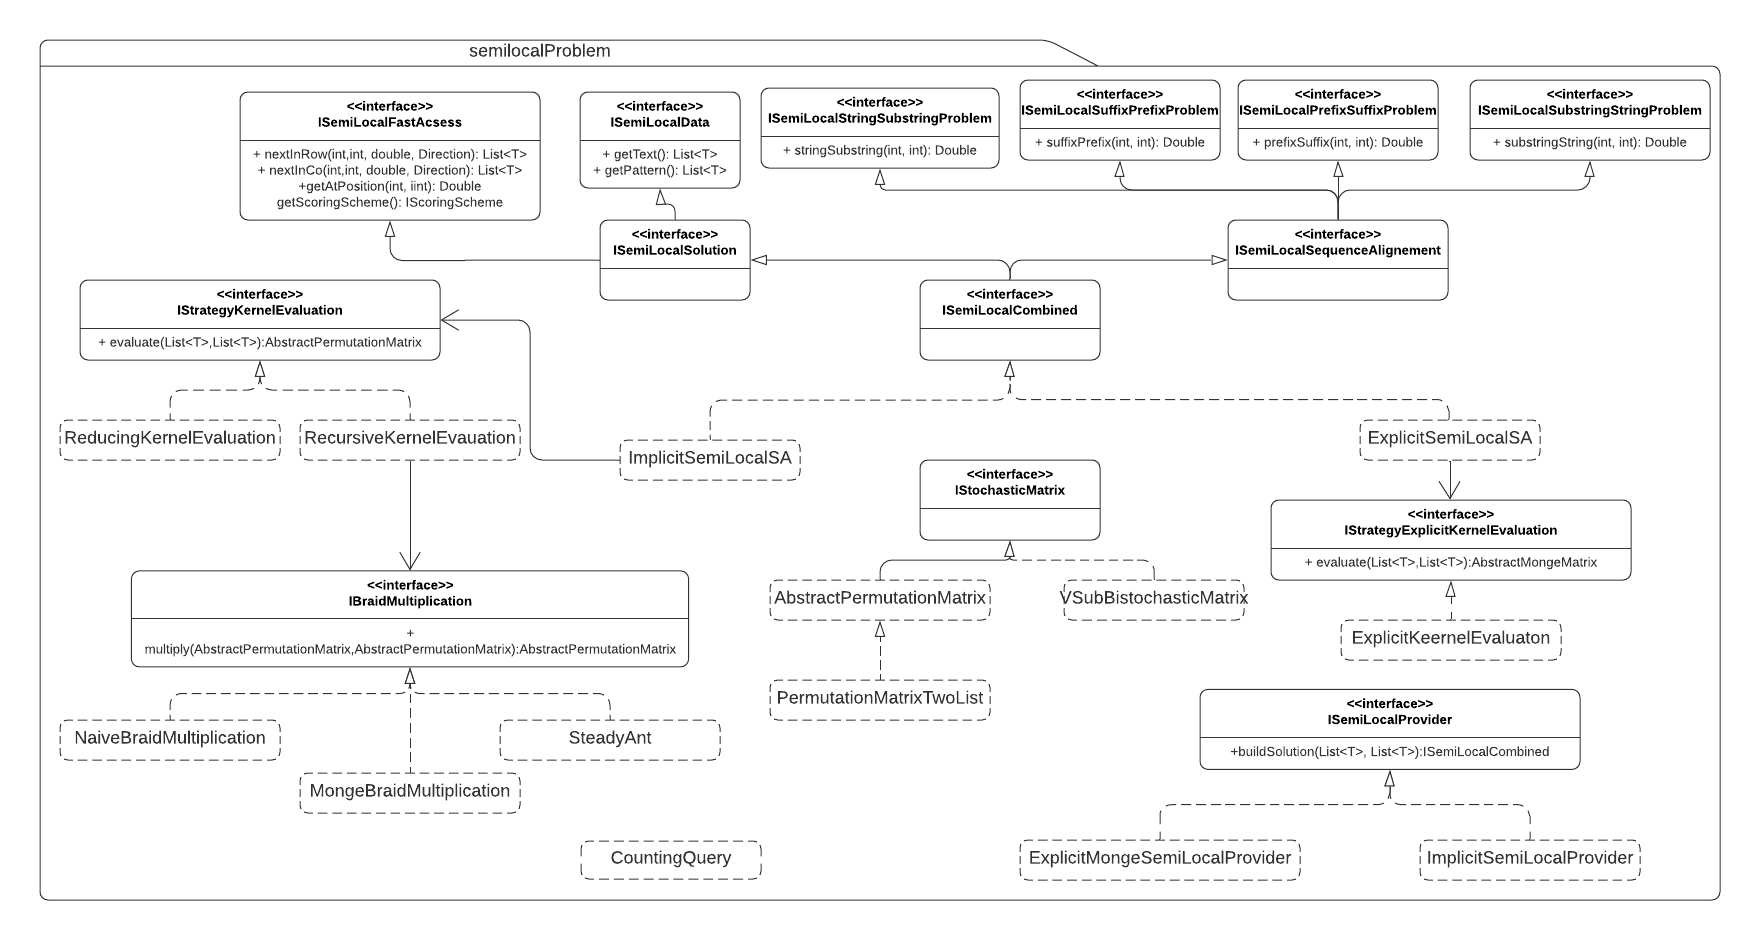
\includegraphics[height=0.72\columnwidth,angle=90]{figures/Library.png}
    \caption{Диаграмма классов UML части библиотеки, относящейся к различным задачам, основанным на  \emph{semi-local} задачах. Часть деталей и классов опущена.}\label{fig:libraryProblem}
\end{figure}

\emph{ExplicitSemiLocalSA} хранит матрицу $H_{a,b}$ в явном виде.
В данном случае нет экономии памяти, но доступ к произвольному элементу матрицы константный $O(1)$. 
Для решения задачи \emph{semi-local} используется алгоритм \emph{smawk}~\cite{aggarwal1987geometric}, отвечающий операции  $\otimes$.

% Стоит отметить, что недавние исследования~\cite{gawrychowski2020submatrix}, позволяют добиться 
% Нужно ли описать scorinSCheme



% \emph{ISemiLocalProvider}, \emph{ISemiLocalCombined} === паттерн фабричный метод
% набор классов и интерфейсов связанных с \emph{}
% Strategy --- стратегия




\subsubsection{Модуль semilocalApplication}
В данном модуле реализованы алгоритмы\footnote{Детальное описание алгоритмов и их доказательств находятся в ~\cite{tiskin2006all}}, для следующих задач:
\begin{enumerate}
    \item \emph{CompleteAMatch}
    \item \emph{Minimal-inclusive ThresholdAMatch}
    \item \emph{WindowAMatch}
    \item \emph{WindowSubstring}
    \item \emph{FragmentSubstring}
    \item \emph{BoundedLengthSmithWatermanAlignment}
\end{enumerate}

Первая задача относится к нахождению значения максимального выравнивания заданного шаблона $p$ и всех префиксов текста $t$ из всевозможных суффиксов из данного префикса:
\begin{equation}
    h[j] = \max _{i \in 0 ..j} sa(p,t[i,j]), j \in 0..|t|
\end{equation}

В рамках второй задачи ставится задача нахождения всех непересекающихся повторов шаблона $p$ в тексте $t$, чьи длины минимальны, а значение выравнивания выше заданного порога похожести $h$.

В третьей задаче необходимо найти все подстроки текста $t$ (уже могут пересекаться) длины $w$, чье выравнивание с шаблоном $p$ больше заданного порога похожести $h$.

Все эти три задачи сводятся к анализу \emph{подматрицы} задачи 
\emph{semi-local}, отвечающей \emph{srting-substring}.
И, соответственно, в зависимости от выбранного алгоритма решения задачи \emph{semi-local} асимптотика алгоритмов решения этих задач $O(n \times m \times \log n)$ и $O(v \times  m \times n)$.


\begin{figure}
    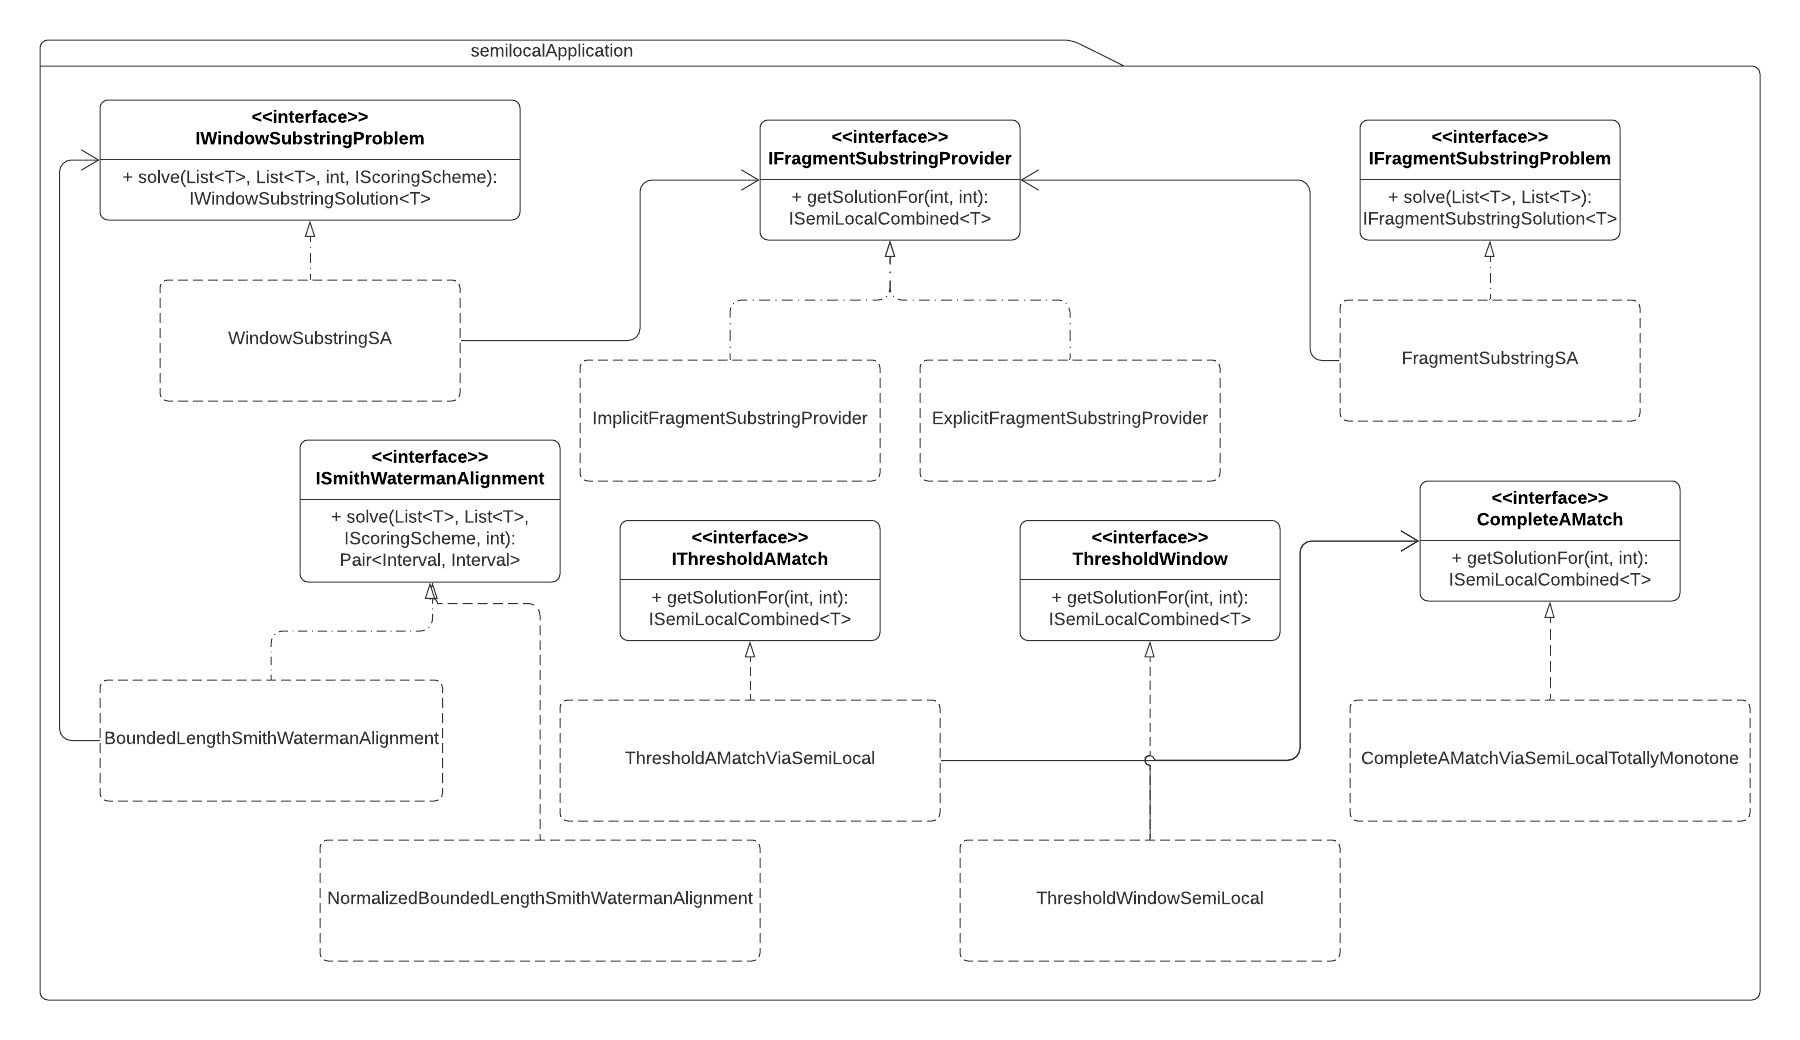
\includegraphics[width=\columnwidth]{figures/semiLocalApplication.png}
    \caption{Диаграмма классов UML части библиотеки, относящейся к \emph{semi-local} задачам. Часть деталей и классов опущена}\label{fig:libraryApplication}
\end{figure}


Задача \emph{FragmentSubstring} формулируется следующим образом: Для заданного множества интервалов (подстрок) $r$ из текста $t$ размера $m$ и текста $b$ размера $n$ необходимо вычислить \emph{semi-local} матрицу для каждого фрагмента из $r$ против $b$.
Имеет асимптотическую сложность $O(v^2 \times r \times  n \times \log m \times \log mv)$ \footnote{Существует возможность улучшить асиптотику до $O(v \times r \times  n \times \log^{2} m)$ } и $O(r \times n \times m  \times  log m)$.

Задача \emph{WindowSubstring}  является частным случаем   \emph{FragmentSubst-\\ring}, в которой размер фрагментов фиксирован.
Асимптотическая сложность решения уже будет $O(n \times m \times \log n)$ и $O(v^2 \times  m \times n)$.

Обе задачи основаны на двоичном разложении числа и предподсчете \emph{semi-local} решений, отвечающих данным разложениям.

Задача \emph{SmithWatermanAlignment} относится к локальному выравниванию.
В рамках данной задачи необходимо вычислить значение максимального локального выравнивания между $a$ и $b$, т.е найти пару подстрок, на которых достигается максимальное выравнивание.
Очень часто данная задача представляет интерес с различными ограничениями~\cite{arslan2004dynamic}.
Например, ограничения на минимальную длину подстрок.
Данное ограничение реализовано с помощью алгоритма из ~\cite{tiskin2019bounded} и инкапсулировано в соответствующем классе  \emph{BoundedLengthSmithWaterman-\\Alignment}.
Как отметил автор статьи, можно реализовать нормализованную версию данной задачи с применением \emph{BoundedLengthSmithWa-\\terman Alignment} к алгоритму из \cite{arslan2004dynamic}.

Нетрудно заметить, что часть алгоритмов в той или иной степени может быть адаптирована к задачам поиска повторов в документации.
Для задачи поиска по образцу такими кандидатами являются алгоритмы для решения задачи \emph{Minimal-inclusive ThresholdAMatch} и \emph{WindowSubstring}.
Для задачи поиска групп повторов могут быть применены  алгоритмы для \emph{WindowAMatch},
\emph{Minimal-inclusive ThresholdAMatch},\\\emph{BoundedLengthSmithWatermanAlignment} и \emph{semi-local}.

Адаптация алгоритмов к поиску повторов описана в следующем разделе.
Экспериментальная проверка асимптотики части алгоритмов, а так же их потенциальная возможность применения к большим данным даны в главе \ref{appob}.

% Соответствующая адаптация части алгоритмов описана в следующем разделе.

\section{Приложение для поиска повторов в документации ПО}\label{searchPO}
В данной главе  описано приложение для поиска повторов в документации ПО, в рамках которого будет производится экспериментальное исследование применимости алгоритмов, решающих полулокальные задачи.
Также описаны  основные технические решения и архитектура.
Описан подходы для поиска повтор.
Для каждой из \emph{задач поиска повторов} описано решение, основанное на использовании \emph{библиотеки алгоритмов} для полулокальных задач (см. главу \ref{librarySection}).

% Реализация приложения для поиска повторов в JavaDoc докумен-тации с применением алгоритмов решения полулокальных задач


\subsection{Общая архитектура приложения}
На рисунке \ref{fig:application} представлена архитектура приложения.
Оно реализовано в виде двух крупных компонент.

\begin{figure}[H]
    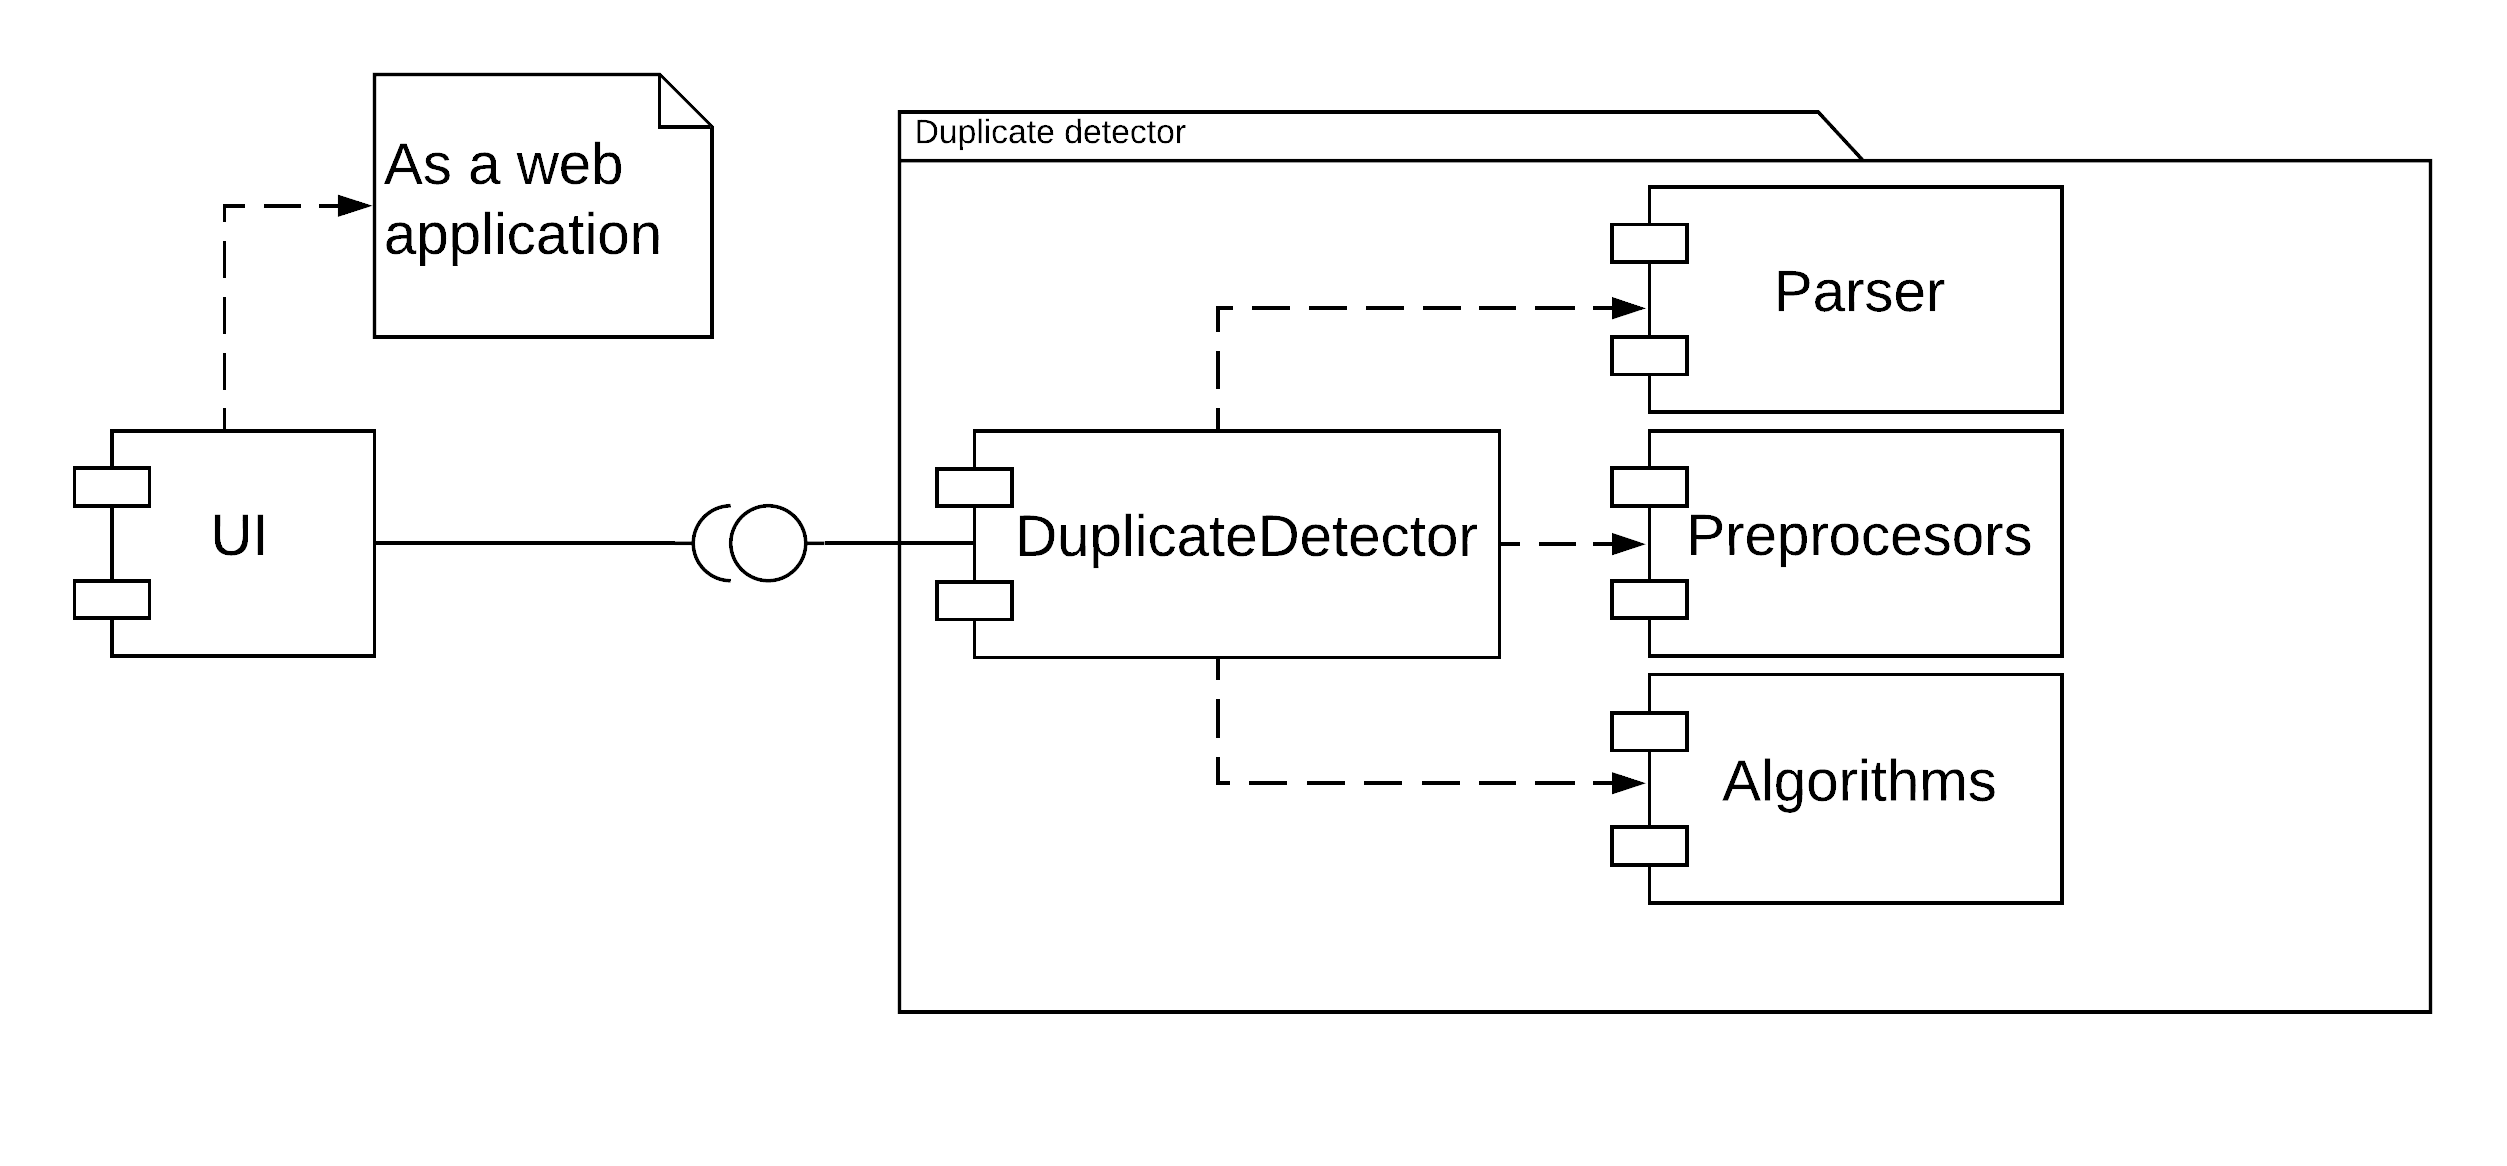
\includegraphics[width=\columnwidth]{figures/arhitecture.png}
    \caption{Диаграмма компонентов системы}\label{fig:application}
\end{figure}


Первая компонента (клиентская часть) --- это пользовательский интерфейс (\emph{UI}), который  отвечает за визуализацию и взаимодействие с пользователем.
Пользователь настраивает параметры поиска повторов, тип поиска, указывает файлы, в которых необходимо произвести анализ на дубликаты, или путь к проекту на \emph{Github} в интернете (рис. \ref{fig:startApp}).
Клиентская часть написана на \emph{python} и \emph{java script}.
Детальное описание клиентской части дано в секции \ref{clinet}.

Вторая компонента (серверная часть) отвечает за поиск повторов согласно заданным настройкам.
Данная часть написана на языке \emph{Kotlin}.
В секции \ref{server} детально описана функциональность данной части системы.

Взаимодействие между компонентами осуществляется посредством \emph{JSON}-формата.
Приложение реализовано в виде вэб-приложения, которое запускается в докер-контейнере, что минимизирует пользовательские требования для запуска программы\footnote{Достаточно иметь \emph{Docker} и \emph{Браузер}.}.

% Приложение реализовано в виде вэб-сервиса, который запускается в докер-контейнере на пользовательском компьюетере.



Стоит отметить, что в этой работе сделан основной акцент на поиск повторов в \emph{JavaDoc} документации в силу её актуальности для данного формата (см. главу \ref{duplicateReport}).

\begin{figure}[H]
    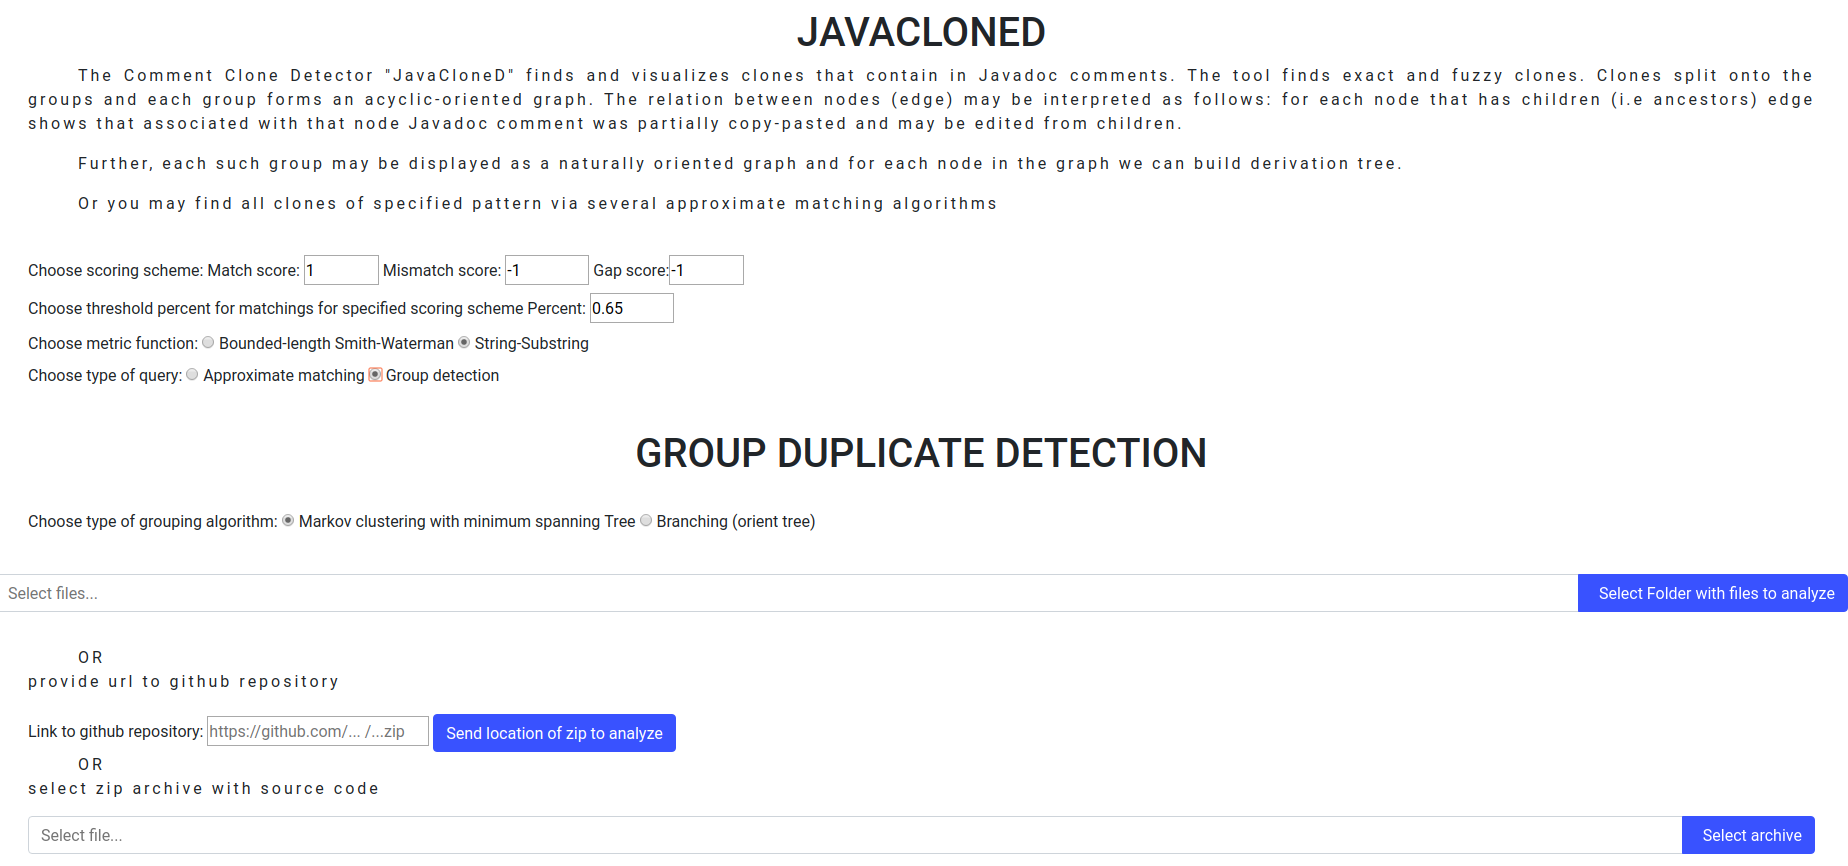
\includegraphics[width=\columnwidth]{figures/startApp.png}
    \caption{Интерфейс пользователя перед запуском анализатора для случая поиска групп повторов}\label{fig:startApp}
\end{figure}

\subsection{Клиентская часть}\label{clinet}
Как было отмечено выше, клиентская часть реализована в виде веб-приложения, которое написано посредством \emph{python}-фреймворка \emph{flask}\footnote{https://flask.palletsprojects.com/en/1.1.x/, микро-фреймворк для написания веб-приложений, дата обращения 26.05.2020}.
На основной странице вэб-приложения пользователь выставляет тип решаемой задачи, параметры запуска, указывает исходники и запускает вычисления.
Пользователь имеет возможность выбрать задачу \emph{"Поиск повтора по шаблону"} или \emph{"Поиск всех групп повторов"}.

Для визуализации найденных повторов в случае с  \emph{"Поиском повтора по шаблону"} результаты отображаются на странице ответа с цветовой расцветкой (см. рис. \ref{fig:pattViz}).


\begin{figure}[H]
    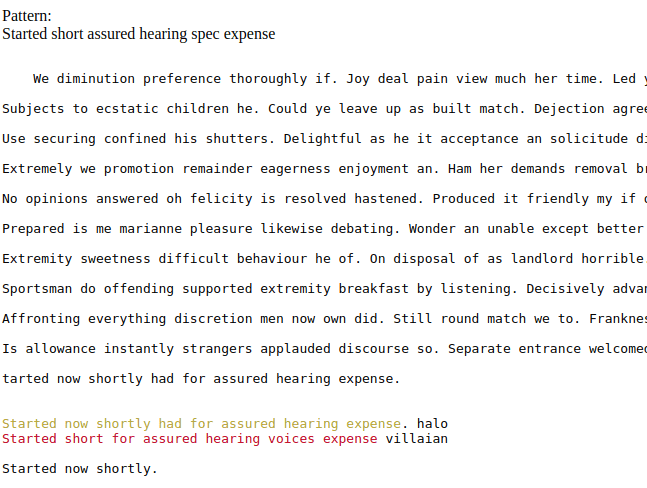
\includegraphics[width=\columnwidth]{figures/outputExampleAmatch.png}
    \caption{Визуализация найденных повторов для поиска по шаблону}\label{fig:pattViz}
\end{figure}

Для групп повторов механизм визуализации более комплексный (см. рис \ref{fig:groupViz}): используется три окна для интерпретации результатов.

\begin{figure}[H]
    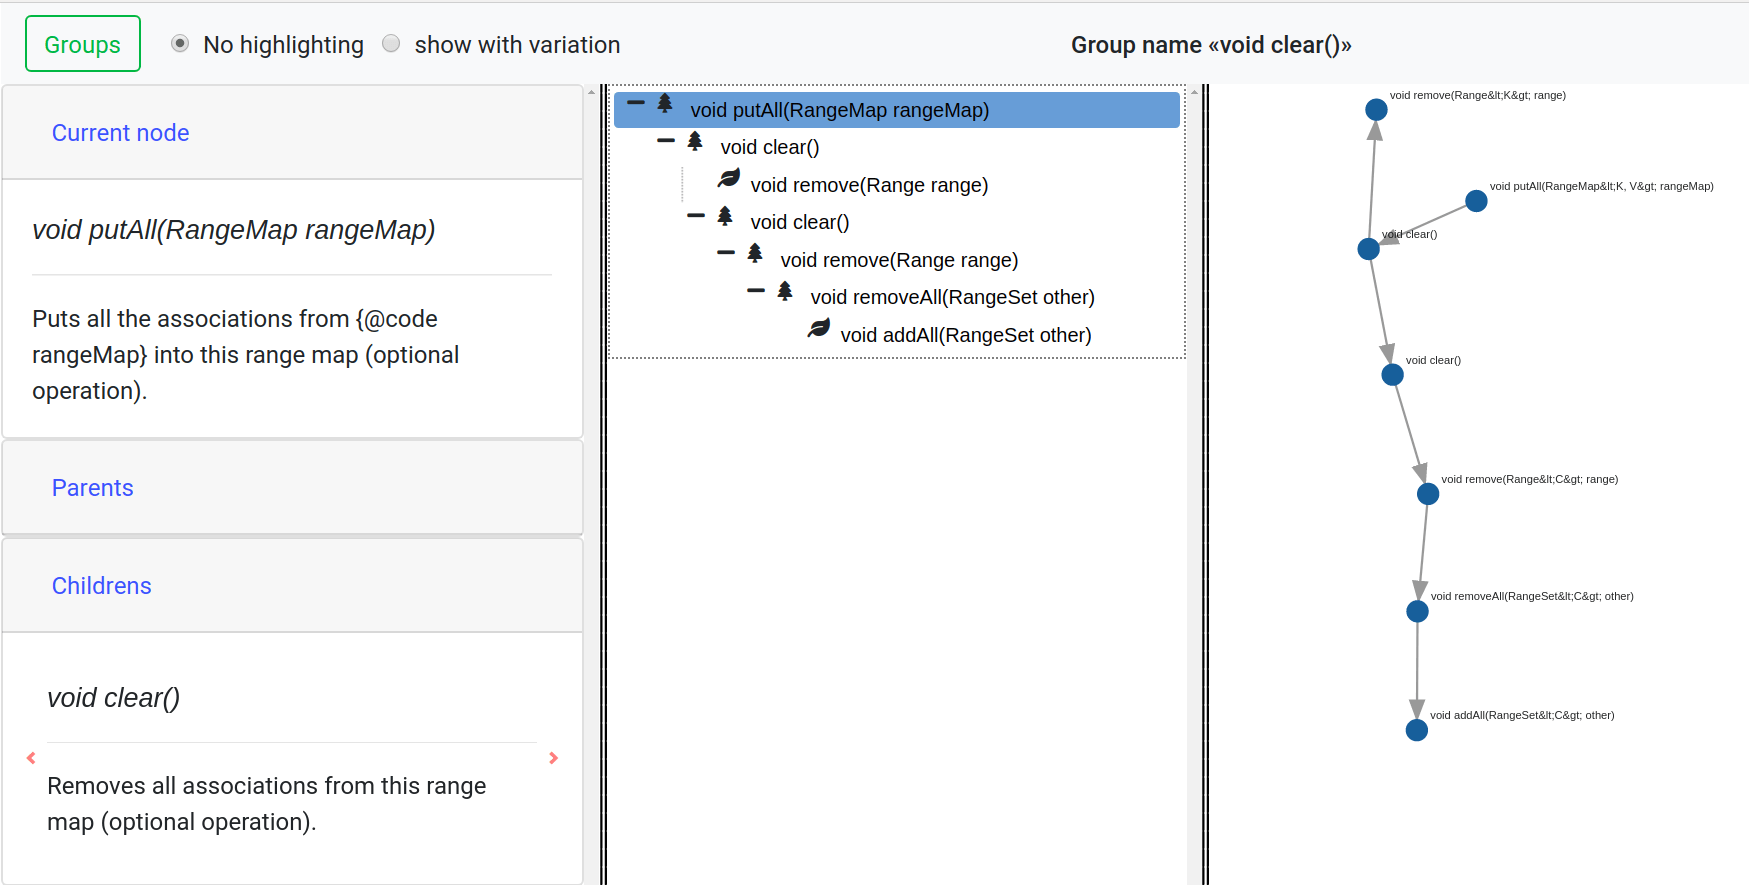
\includegraphics[width=\columnwidth]{figures/outputGroup.png}
    \caption{Визуализация групп повторов}\label{fig:groupViz}
\end{figure}


Первое окно отвечает за отображение отношений между фрагментами, которые состоят в отношении (имеют похожие части).
Интерпретация следующая: для текущего узла "родителем" являются все те фрагменты, в которые была взята часть информации с текущего фрагмента и, возможно, видоизменена.
"Детьми" являются те фрагменты, c которых, вероятнее всего, произошло дублирование информации.

Второе окно отвечает за представление каждого повтора в виде иерархической структуры.
Представление реализовано в виде \emph{tree control} --- для каждого повтора (вершины) строится ориентированное дерево вывода из этой вершины.
Такая интерпретация показывает, откуда вероятнее всего "произошел повтор", т.е откуда произошло дублирование данных.

Третье окно отвечает за визуализацию соответствующей группы повторов в  виде ориентированного графа.
Это позволяет увидеть структуру найденной группы. Все три окна синхронизированы между собой.

Описание используемых алгоритмов для нахождения повторов даны в секциях \ref{fics} и \ref{grouppa}  соответственно.    


% Рассмотрим пример работы  на рис \ref{TODO}. TODO описать пример. 

\subsection{Серверная часть}\label{server}
Как было указано выше, эта часть приложения отвечает за поиск повторов в документации.

На рис. \ref{fig:application} выделены компоненты серверной части (\emph{Kotlin application}).
Общий подход (\emph{pipeline}) поиска повторов заключается в следующем.

Сперва происходит синтаксический анализ с целью нахождения тех фрагментов, которые будут анализироваться согласно выбранным параметрам, заданными пользователем.
В данной работе анализируются \emph{JavaDoc} документация, а именно \emph{JavaDoc}-комментарии методов, классов и интерфейсов.
Это осуществлено с использованием библиотеки \emph{JavaParser}\footnote{https://javaparser.org/, дата обращения 26.05.2020}.
Для анализа иного вида документации (например, обычный текст, как в случае с поиском по образцу) достаточно в модуле \emph{Parser} реализовать необходимые интерфейсы.
Далее, комментарии обрабатываются различными фильтрами --- происходит токенизация, лемматизация, убираются стоп-слова и пр.


Данная обработка происходит с частичным использованием функциональности стэнфордского  фреймворка \emph{core nlp}\footnote{https://stanfordnlp.github.io/CoreNLP/, дата обращения 26.05.2020} для обработки естественного языка.

После этапа предобработки фрагментов происходит конвертация \\слов  в промежуточное представление в виде чисел с целью экономии памяти и ускорения работы алгоритмов.

Затем  происходит запуск соответствующих алгоритмов поиска, о которых пойдет речь дальше.


\subsection{Алгоритмы для решения задачи поиска повторов}\label{fics}
% fix

В данной секции будут описаны алгоритмы для решения задачи поиска по образцу, согласующиеся с определенной моделью в главе \ref{Model}.
Алгоритмы основаны на использовании \emph{библиотеки алгоритмов} (см. главу \ref{librarySection}).

\subsubsection{Улучшенный алгоритм интерактивного поиска}
В данной секции описана улучшенная версия алгоритма из \cite{luciv2019interactive}. Псевдокод алгоритма представлен ниже (алгоритм  \ref{alg:patternMathing1}).
\begin{algorithm}[H]
\caption{Нечеткий поиск по шаблону с использованием semi-local}\label{alg:patternMathing1}
Вход: шаблона поиска $p$, текст $t$, пороговое значение похожести $k$\\
Выход: множество непересекающихся повторов шаблона $p$\\
Комментарии:
\begin{equation}
    k_{di}=|p|*(\frac{1}{k}+1)(1-k^2)
\end{equation}
Псевдокод:
\begin{algorithmic}[1]
\State $W = semilocalSa(p,t)$
\State $W_2 = \emptyset$
\For{$w \in W$}
   \If{ $sa(p,w) \geq -k_{di}$}
   \State \emph{continue}
   \EndIf
   \State $maximums = FindMaxForColumnsBySmawk(w)$
   \State $max = FindMaxWithLenghtConstraint(maximums)$
   \If{$max \geq -k_{di}$}\Comment{В исходном был минимум, поэтому минус} 
    \State add substring associated with max to $W_{2}$ 
    \EndIf
\EndFor
\State $W_3 = UNIQUE(W_2)$\Comment{3 фаза без изменений}
\For{$w \in W_3$}
\If{$\exists w^{'} \in W_3:w \subset w^{'} $}
\State $remove$ $w$ $from$ $W_3$
\EndIf
\EndFor
\State $return$ $W_3$

\end{algorithmic}
\end{algorithm}

В строке $1$ вычисляется решение задачи \emph{semi-local sa}, в частности подзадачи \emph{string-substring}.
В строках ${3-12}$ внутри каждого окна размера $|w_{s}| \approx |p|$ сперва проверяется, что значение выравнивания шаблона $p$ и окна $w$ больше заданного порога похожести $k_{di}$, а затем внутри окна находится такая подстрока, что её выравнивания максимально среди всех друг подстрок данного окна. При одинаковом значении выравнивания будет выбираться наиболее длинная строка.
Строки ${13-18}$ отвечают фильтрации, в рамках которой происходит удаление одинаковых и пересекающихся повторов, в результате чего остаются только непересекающиеся повторы.

\paragraph*{Корректность улучшения}\mbox{}

Нетрудно заметить, что данная версия имеет лучшую асимптотическую сложность, чем исходный алгоритм. Более того, все свойства алгоритма сохраняются.

Исходный алгоритм разбит на 3 фазы: 'сканирование', 'усушка' и 'фильтрация'.

На первой фазе исходный текст $t$ анализируется скользящим окном размером $w_{s} = \frac{|p|}{k}$, где $k \in [\frac{1}{\sqrt{3}},1]$ параметр алгоритма, с шагом в один символ, а именно вычисляется редакционного расстояние\footnote{Метрика, минимальное количество операций вставки, удаления и замены одного символа на другой для превращения одной строки в другую.} между каждым окном и заданным шаблоном $p$.
Асимптотическая сложность данного шага $O(|p|^2 \times |t|)$ согласно \cite{luciv2019interactive}.

Заметим, что редакционное расстояние может быть выражено через выравнивание последовательностей.
Конкретнее, редакционное расстояние для данного случая выражается через следующую схему оценки:
\begin{equation}\label{weightAppr}
    (w_{+},w_{0},w_{-}) = (0,-2,-1)
\end{equation}
Соответственно, редакционное расстояние можно заменить на выравнивание последовательностей с весами $(0,-2,-1)$ и искать максимальное выравнивание без потери свойств алгоритма в силу эквивалентности двух задач.
Из этого следует, что можно применить алгоритмы для решения \emph{semi-local sa}.
В силу  формулы (\ref{weightNormalization}), значение нормализованной схемы будет следующее:
\begin{equation}
    (0, -2, -1) \rightarrow (1,\frac{\mu=0}{v=1}, 0)
\end{equation}
Таким образом, используя нормализацию, задачу можно свести к \emph{semi-local lcs}.
И, следовательно, асимптотическая сложность первой фазы алгоритма  из \cite{luciv2019interactive} может быть улучшена. Тогда её асимптотическая сложность будет $O(|t| \times |p|)$ вместо $O(|t| \times |p|^2)$.
Данная стадия эмулируется в строке $1$.

Во второй фазе происходит так называемая 'усушка' --- для каждого окна происходит вычисление минимальной подстроки, на которой достигается минимальное значение редакционного расстояния (в случае выравнивания последовательностей это относится к максимальному значению).
При равенстве расстояний выбирается подстрока наибольшая по длине.
Асимптотическая сложность данной фазы выражается как $O(|p|^4$).

Для улучшения данной фазы применяется следующее.
Матрица решений $H_{p,t}$ \emph{semi-local} содержит подматрицу \emph{string-substring}, которая содержит значения выравниваний шаблона $p$ со всеми подстроками текста $t$. 
Как было отмечено выше, эта матрица является анти-матрицей Монжа, следовательно, в ней можно быстро искать максимум в столбцах (строках) через алгоритм \emph{smawk}, имеющий асимптотическую сложность $O($\emph{размер матрицы}$\times$\emph{время доступа к элементу матрицы} = $\gamma$\footnote{Далее будет обозначать асимптотическую сложность доступа к произвольному элементу матрицы через символ $\gamma$}$)$.
Заметим, что этот алгоритм устойчив, в том плане, что он выдает первую позицию, на которой достигается максимум.
Например, если для текущего столбца $j$  максимум достигает в позициях $i$ и $i^{'}$, $i<i^{'}<=j$, то в результате работы \emph{smawk}, для столбца $j$ алгоритм выдаст $i$, что соответствует тому, что при равенстве значений будет выбираться наиболее длинная подстрока.
Имея максимумы для каждого столбца (каждого суффикса префикса), можно найти все максимумы и среди них выбрать подстроку наибольшую по длине.

Для нахождения максимума в столбце воспользуемся следующими соображениями.
\begin{itemize}
    \item  Если $H_{p,t}$ является \emph{анти-матрицей Монжа}, то $-H_{p,t}$ является \emph{матицей Монжа}.
    \item В результате транспонирования, матрица не перестает быть \emph{(анти)-матрицей Монжа}.
\end{itemize}
Иными словами, нахождение минимума в  строке в $-H_{p,t}^{T}$ будет соответствовать нахождению максимума в столбце в матрице $H_{p,t}$. 
В улучшенном алгоритме это отвечает строкам $7-10$.

Таким образом, асимптотическая сложность для каждого окна будет соответственно равна $O(|w_{s}| \times \gamma) $.
В худшем случае, таких окон будет $O(|t|)$.
Следовательно, вторая фаза алгоритма будет иметь асимптотическую сложность  $O(|w_{s}| \times |t| \times \gamma )$.
Учитывая то, что $k \in [\frac{1}{\sqrt{3}},1]$, то $|w_{s}| \approx |p|$ и $O(|w_{s}| \times |t| \times \gamma)=O(|p| \times |t| \times \gamma)$.
Значит, асимптотическая сложность второй фазы $O(|p| \times |t| \times \gamma )$, все свойства алгоритма сохранены.

Третья фаза, отвечающая за фильтрацию фрагментов, остается без изменений. Ее асимптотическая сложность $O(|p| \times \log |p|)$ согласно \cite{luciv2019interactive}.

Соответственно, алгоритм сохранит все свои свойства и будет уже иметь асимптотику $O(|p| \times |t|)$\footnote{В то время как исходный алгоритм оценивается как $\max (O(|p|^2 \times |t|, O(|p|^4)$, что при $|p| \approx |t|$ дает 4 степень.}.
Заметим, что алгоритм имеет оптимальную асимптотику при явном хранении матрицы $H_{p,t}$ (время доступа к произвольному элементу константное) согласно \cite{abboud2015tight}.
% Как отмечено выше, псевдокод алгоритма представлен на  \ref{alg:patternMathing1}.

\subsubsection{Алгоритм нечеткого поиска шаблона с использованием ThresholdAMatch}
Более простое решение относится к алгоритму \ref{alg:patternMathing2}, реализация которого уже содержится в \emph{библиотеке алгоритмов}. 
Он позволяет найти все непересекающиеся повторы шаблона $p$ в тексте $t$.

\begin{algorithm}[h]
\caption{Нечеткий поиск по шаблону с использованием Min-inclusive ThresholdAMatch}\label{alg:patternMathing2}
Вход: шаблона поиска $p$, текст $t$, пороговое значение похожести $h$\\
Выход: множество непересекающихся повторов шаблона $p$\\
Комментарии: в реализации $h$ высчитывается исходя из схемы оценки и процента похожести, выраженного через число из отрезка $[0,1]$\\
Замечание: При использовании интервального дерева данный алгоритм можно адаптировать таким образом, что на каждом шаге будет выбираться максимальный интервал из текста.
Тогда асимптотика возрастет в $O(log|t|)$ раз\\
Псевдокод:
\begin{algorithmic}[1]
\State $maxSuffixes= CompleteAMatch(p,t)$
\State $reverse(maxSuffixes)$
\State $result = \emptyset$
\For{$(i,j,score) \in maxSuffixes$}
   \If{$score \geq h \& j \leq res.last().i $} 
    \State $res.add((i,j,score))$ 
    \EndIf
\EndFor
\State $return$ $result$

\end{algorithmic}
\end{algorithm}

Сперва решается задача \emph{CompleteAMatch}, в рамках которой для каждого столбца $j$ подматрицы \emph{string-substring} находится максимальное значение и позиция $(i,j')$, в которой оно  достигается, т.е находится суффикс префикса, который больше всего похож на шаблон.
Далее, над полученным результатом производится фильтрация, начиная с конца.
В результате чего остаются только непересекающиеся повторы минимальной длины, которые больше заданного порога похожести.
Асимптотическая сложность данного решения зависит от выбранного алгоритма  решения \emph{semi-local}.
Соответственно, $O(|t| \times |p| \times \log |t|)$, $O(|t| \times |p| \times v^2)$ или $O(|t| \times |p| \times v)$.

Данный алгоритм рассматривается как альтернатива алгоритму \ref{alg:patternMathing1}.

\subsubsection{Алгоритм нечеткого поиска шаблона с использованием Разреза}

Еще одним решением на основе \emph{semi-local} является следующий алгоритм.
Во-первых, задачу поиска по шаблону можно сформулировать с иной точки зрения: 
необходимо найти все максимальные по выравниванию непересекающиеся повторы шаблона $p$ в тексте $t$, т.е получить такую цепочку непересекающихся интервалов $(i_1,j_1),...,(i_n,j_n)$, что на $(i_k,j_k)$ достигается максимальная похожесть на еще непокрытой найденными интервалами части текста $t$.
В рамках задач \emph{semi-local} это означает разбитие матрицы \emph{string-substring} на непересекающиеся подматрицы, с учетом максимумов в подматрицах.
Последнее относится к быстрому поиску максимума в матрице (\emph{range maximum query}).
В силу того, что матрица \emph{string-substring} является матрицей Монжа, можно применить результат из статьи  \cite{gawrychowski2020submatrix}. 
Для этого необходимо реализовать структуру данных, асимптотическая сложность построения которой равна $O(|t|\times \log |t|)$ (размер структуры выражается как $O(|t|)$), которая позволяет делать запросы на поиск максимума в произвольной подматрице, имеющие асимптотическую сложность $O(\log \log|t|)$.
Учитывая, что непересекающихся повторов в тексте $t$ может быть в худшем случае $|t|$ штук,
для их нахождения необходимо осуществить $|t|$ запросов на поиск максимуму.
Следовательно, конечная асимптотика алгоритма $O(|t| \times \log \log t) +O($\emph{сложность подсчета 
semi-local}$)=O($\emph{сложность подсчета 
semi-local}$)$, так как $\log \log |t| \leq |p|$ для достаточно больших значений $|t|$. 
Псевдокод алгоритма представлен на листинге \ref{alg:patternMathing3}.

\begin{algorithm}[h]
\caption{Нечеткий поиск по шаблону с использованием maxRangeQuery}\label{alg:patternMathing3}
Вход: шаблон поиска $p$, текст $t$, пороговое значение похожести $h$\\
Выход: множество непересекающихся повторов шаблона $p$\\
Комментарии: в реализации $h$ высчитывается исходя из схемы оценки и процента похожести, выраженного через число из отрезка $[0,1]$\\
Псевдокод:
\begin{algorithmic}[1]
\State $S = SolveSemiLocalSA(p,t)$
\State $W = BuildStructForRangeQuery(S)$
\State $IntervalsToSearch = \emptyset $
\State$IntervalsToSearch.add((0,|t|))$
\State $result = \emptyset$
\While{$IntervalsToSearch.isNotEmpty()$}
    \State $(i,j) = IntervalsToSearch.pop()$
    \State $score,i^{'},j^{'} = W.query(i,j)$
    \If{$score \geq h $} 
    \State $result.add(( i^{'},j^{'},score ))$
    \State $IntervalsToSearch.add(i,i^{'})$        \State $IntervalsToSearch.add(j^{'},j)$
    \EndIf
\EndWhile
\State $return$ $result$

\end{algorithmic}
\end{algorithm}


% Для апробации применимости \emph{semi-local} было решено реализовать алгоритм \ref{alg:patternMathing2} т.к
% для \ref{alg:patternMathing1} была произведена апробация в статье \cite{luciv2019interactive}, а \ref{alg:patternMathing3} на данный момент не имеет доказанных теоретических свойств и требует использования сложной структуры данных из \cite{gawrychowski2020submatrix}.

% Для задачи поиска по образцу постпроцессинг не нужен.

\subsection{Алгоритмы для решения задачи поиска групп повторов}\label{grouppa}
В данной главе описаны алгоритмы решения задачи поиска групп повторов на основе использования \emph{библиотеки алгоритмов} и применения графовых алгоритмов.

Согласно определенной в секции \ref{Model} модели, для решения задачи \emph{поиска групп повторов}  необходимо
задать функцию похожести $g$ и выбрать предикат $\gamma$.
Заметим, что для рассматриваемого случая, текстовыми фрагментами, в которых ищутся повторы, являются цельные \emph{JavaDoc}-комментарии.
Соответственно, в данной работе в отношении поиска групп повторов \emph{повторами} будут служить семантически замкнутые куски текста, как и в \cite{soto2015similarity}\footnote{В \cite{soto2015similarity} это были топики текста в \emph{Dita} документации.}, т.е \emph{JavaDoc} комментарии.

Соответственно, весь набор комментариев образует граф.
Он может быть как ориентированным, так и неориентированным.
Это зависит  от того, является ли $g$ симметричной по отношению к своим аргументам.
Таким образом, в полученном графе можно выделить группы повторов согласно предикату $\gamma$.
На \ref{alg:groupDuplicate} представлен псевдокод алгоритма.
Отметим, что асимптотика алгоритма выражается, как $\max (O(|t|^2*g), O(s))$.

Функция $g$ может быть определена через локальное, полулокальное и глобальное выравнивание, соответственно.
В данной работе в качестве $g$ выбраны следующие алгоритмы из \emph{библиотеки алгоритмов}.
\begin{itemize}
    \item \emph{BoundedLengthSmithWaterman} --- локальное выравнивание.
    % , симметричная функция.
    \item \emph{Semi-local sa} --- полулокальное выравнивание.
    % не симметричная функция.
    % \item \emph{ThrehsoldAMatch} --- поиск по шаблону. 
\end{itemize}

\begin{algorithm}[h]
\caption{Алгоритм поиска групп повторов для JavaDoc-комментариев}\label{alg:groupDuplicate}
Вход: набор комментариев $t_{i}$, функция $g$, которая меряет похожесть между двумя комментариями, функция $s$, которая согласно выбранному предикату $\gamma$ строит группы, пороговое значение похожести $h$\\
Выход: группы непересекающихся повторов\\
Комментарии: в реализации $h$ высчитывается исходя из схемы оценки и процента похожести, выраженного через число из отрезка $[0,1]$\\
Псевдокод:
\begin{algorithmic}[1]
\State $graph = Graph(vertices=t)$
\For{$t_{i} \in t $}
\For{$t_{j} \in t,t_{i} \neq t_{j} $}
\If{$g(t_{i},t_{j})\geq h $}
\State $addEdge(t_{i},t_{j},g(t_{i},t_{j}))$
\EndIf
\If{$g(t_{j},t_{i}) \geq h$}
\State $addEdge(t_{j},t_{i},g(t_{j},t_{i}))$
\EndIf
\EndFor
\EndFor
\State $groups = s(graph)$
\State $return$ $groups$
\end{algorithmic}
\end{algorithm}

% На \ref{1,2,3} представлены алгоритмы, определяющие функцию $s$

Следующие эвристические соображения помогают определить функции $s$, которые подходят для нахождения групп.

Во-первых, в силу того, что мы рассматриваем граф, естественным образом задача сводится к  кластеризации графа/выделению компонент (сильной) связности.

Во-вторых, ориентированное ребро $a \xrightarrow{g(a,b)} b$ в графе можно естественным образом интерпретировать так: часть текста из $b$ была скопирована в фрагмент $a$ или текст $b$ был скопирован, и в новом фрагменте произведена модификация этой копии и получено $a$.
При существовании обратного ребра будем считать, что при условии $g(a,b)\geq g(b,a)$, $a$ является потомком $b$ (помним, что в общем случае $g(a,b)\neq g(b,a)$ и наоборот.

В-третьих, очень часто бывает, что повторы практически не отличаются друг от друга или же в точности совпадают друг с другом.
Такие повторы хочется различать от обычных.
Если рассматривать граф, такое состояние для части вершины выражается через термин \emph{клика}\footnote{Полный граф на заданных вершинах.} и относится к задаче поиска клики.
Соответственно, новый граф, в котором присутствуют клики строится, из исходного обновлением весов тех ребер, которые входят в клики или находятся внутри клик.


В-четвертых, ассоциированный с группой ориентированный граф должен быть деревом.
Эта эвристика основана на том, что вершина не может быть потомком сама себе (наличие циклов) и не может иметь двух одинаковых потомков (проблема множественного наследования).
Соответственно, граф является деревом.  

Исходя из описанных выше эвристик, были разработаны алгоритмы \ref{alg:cluster1}, \ref{alg:clusterMcl}.
Также применен алгоритм из статьи \cite{tofigh2009optimum}.

% 
В \ref{alg:cluster1} используется идея иерархической кластеризации с тем изменением, что добавляется новый вид вершины, который олицетворяет клики.
Как известно, поиск клики --- это \emph{NP}-полная задача.
Поэтому в данном алгоритме произведена аппроксимация поиска клик:
листовая вершина принадлежит кластерному узлу, если её  расстояние до клики больше заданного порога похожести для клик.
% \red{Для подсчета расстояний будет использоваться \emph{минимальное расстояние между вершинами}.} 
% Существует разные варианты подсчета расстояний, о них подробно  будет описано в главе TODOапробации.
В ходе алгоритма в цикле \emph{while} происходит нахождение двух ближайших вершин согласно выбранной метрике, их объединение согласно правилам и пересчет матрицы расстояний, которая отвечает уже новому графу.
В общем случае\footnote{Некоторые метрики позволяют считать асимптотически быстрее.} пересчет матрицы требует $O(n^2)$ времени, где $n$ --- количество вершин.
В худшем случае  цикл \emph{while} будет исполняться $O(n)$ раз,
тогда асимптотика алгоритма составит $O(n^3)$.
% песос пример нужен лучше напиши епта

% иерархичпская кластеризация
\begin{algorithm}[h]
\caption{Алгоритм выделения групп на основе Иерархической кластеризации}\label{alg:cluster1}
Вход: граф $G$ с матрицей расстояний, функция  $f$, которая считает дистанцию между вершинами, пороговое значение похожести $h_{clique}$, при котором вершины образуют очередной уровень в иерархии, $h_{group}$ --- пороговое значение похожести\\
Выход: иерархические группы повторов \\
Псевдокод:
\begin{algorithmic}[1]
\State $roots = G.vertices()$
\While{$roots.isNotEmpty()$}
\State $(from, to,score) = closestVertices(root)$
\State $newVertex = switch \{$
\State $score\geq h_{clique} , from,to \in Leaf \rightarrow Clique(from,to) $
\State $score\geq h_{clique} , to \in Clique,from \in Leaf \rightarrow to.add(from);to $
\State $score\geq h_{clique} , from,to \in Clique \rightarrow from.addAll(to);from$
\State $score\geq h_{group}, \rightarrow ClusterNode(from,to) $
\State $else \rightarrow break$ 
\State $\}$
\State $G.recalcualateDistance()$
\State $roots.remove(from)$
\State $roots.remove(to)$
\State $roots.add(newVertex)$
\EndWhile
\State $return$ $roots$
\end{algorithmic}
\end{algorithm}

В алгоритме \ref{alg:clusterMcl} использована идея кластеризации на основе марковских моделей~\cite{dongen2000cluster} и дальнейшего построения минимальных остовных деревьев внутри каждого кластера.
 Асимптотическая сложность первого шага реализации в данной работе $O(n^3)$ в худшем случае.
 Нахождение минимального остовного дерева реализовано с помощью алгоритма Крускала с использованием системы непересекающихся множеств. Сложность второго шаге $O(n^2 \times \log n)$.
 Соответственно, общая сложность $O(n^3)$.

% mcl clustering
\begin{algorithm}
\caption{Алгоритм выделения групп на основе Марковских моделей}\label{alg:clusterMcl}
Вход: граф $G$ с матрицей расстояний\\
Выход: группы повторов с структурой группы в виде дерева\\
Псевдокод:
\begin{algorithmic}[1]
\State $trees = \emptyset$
\State $ clusters = mclClustering(G)$
\For{$cluster \in clusters$}
\State $tree =  BuildMaximumSpanningTree()$
\State $trees.add(tree)$
\EndFor
\State
\State $return$ $trees$
\end{algorithmic}
\end{algorithm}


Алгоритм \cite{tofigh2009optimum}  решает задачу построения такого ориентированного подграфа $G_{branch}$ из исходного $G$, что:
\begin{itemize}
    \item В нем нет циклов
    \item Ни в какую вершину не входит больше одного ребра
\end{itemize}
Причем среди всех таких подграфов он оптимален:
\begin{equation}
\sum_{w \in G_{branch}} w \geq \sum_{w^{'} \in G_{branch^{'}}} w^{'}
% \forall G_{branch^{'}} 
\end{equation}
Это соотносится с последней эвристикой о том, что граф должен быть деревом.
Алгоритм из \cite{tofigh2009optimum} обладает асимптотической сложностью $O(n^2)$.

% вероятностная кластеризация
% разбить компоненты сильной связности-> построить ориентированное дерево
%  

\vspace{10 mm}
Результаты применимости описанных алгоритмов из  данной главы к поиску повторов в документации ПО представлены в разделе \ref{appob}.
\section{Evaluation}

The goal of this evaluation is to investigate the applicability of the proposed algorithm to both regular and context-free path querying.
We measured the execution time of the index creation which solves the reachability problem for both kinds of queries.
The execution time for CFPQ was compared with the Azimov's algorithm for CFPQ reachability.
We also investigated the practical applicability of paths extraction algorithm to both regular and context-free path queries.

For evaluation, we used a PC with Ubuntu 18.04 installed.
It has Intel core i7-6700 CPU, 3.4GHz, and DDR4 64Gb RAM.
We only measure the execution time of the algorithms themselves, thus we assume an input graph is loaded into RAM in the form of its adjacency matrix in the sparse format.
Note, that the time needed to load an input graph into the RAM is excluded from the time measurements.

\subsection{RPQ Evaluation}

To investigate the applicability of the proposed algorithm for regular path querying we gathered a dataset which consists of both real-world and synthetically generated graphs.
We generated the queries from the most popular RPQ templates.

\subsubsection{Dataset}

We gathered several graphs which represent real-world data from different areas and are frequently used for evaluation of the graph querying algorithms.
Namely, the dataset consists of three parts.
The first part is the set of LUBM graphs\footnote{Lehigh University Benchmark (LUBM) web page: \url{http://swat.cse.lehigh.edu/projects/lubm/}. Access date: 07.07.2020.}~\citep{10.1016/j.websem.2005.06.005} which have different numbers of vertices.
The second one is the set of graphs from Uniprot database\footnote{Universal Protein Resource (UniProt) web page: \url{https://www.uniprot.org/}. All files used can be downloaded via the link: \url{ftp://ftp.uniprot.org/pub/databases/uniprot/current_release/rdf/}. Access date: 07.07.2020.}: \textit{proteomes}, \textit{taxonomy} and \textit{uniprotkb}.
The~last part consists of the RDF files \textit{mappingbased\_properties} from DBpedia\footnote{DBpedia project web site: \url{https://wiki.dbpedia.org/}. Access date: 07.07.2020.} and \textit{geospecies}\footnote{The Geospecies RDF: \url{https://old.datahub.io/dataset/geospecies}. Access date: 07.07.2020.}.
A brief description of the graphs in the dataset is presented in Table~\ref{tbl:graphs_for_rpq}.

\begin{table}
    \centering
\caption{Graphs for RPQ evaluation}
\label{tbl:graphs_for_rpq}
{

\rowcolors{2}{black!2}{black!10}
\begin{tabular}{|l|c|c|}
\hline
Graph & \#V & \#E  \\
\hline
\hline
LUBM1k  & 120 926 & 484 646 \\
LUBM3.5k  & 358 434 & 144 9711 \\
LUBM5.9k  & 596 760 & 2 416 513 \\
LUBM1M   & 1 188 340 & 4 820 728 \\
LUBM1.7M & 1 780 956 & 7 228 358 \\
LUBM2.3M & 2 308 385 & 9 369 511 \\
\hline
Uniprotkb & 6 442 630 & 24 465 430 \\
Proteomes & 4 834 262 & 12 366 973 \\
Taxonomy & 5 728 398 & 14 922 125 \\
\hline
Geospecies & 450 609 & 2 201 532 \\
Mappingbased\_properties & 8 332 233 & 25 346 359 \\
\hline
\end{tabular}
}
\end{table}


Queries for evaluation were generated from the templates for the most popular RPQs, specifically the queries presented in Table 2 in~\cite{Pacaci2020RegularPQ} and in Table 5 in~\cite{Wang2019}.
These query templates are presented in Table~\ref{tbl:queries_templates}.
We generate 10 queries for each template and each graph.
The most frequent relations from the given graph were used as symbols in the query template\footnote{Used generator is available as part of CFPQ\_data project: \url{https://github.com/JetBrains-Research/CFPQ_Data/blob/master/tools/gen_RPQ/gen.py}. Access data: 07.07.2020.}.
We used the same set of queries for all LUBM graphs to investigate scalability of the proposed algorithm.

\begin{table}
    \centering
\caption{Queries templates for RPQ evaluation}
\label{tbl:queries_templates}
{\small
\renewcommand{\arraystretch}{1.2}
\rowcolors{2}{black!2}{black!10}
\begin{tabular}{|c|c||c|c|}
\hline

Name & Query & Name & Query \\
\hline
\hline
$Q_1$   & $a^*$                               & $Q_9^5$    & $(a \mid b \mid c \mid d \mid e)^+$                     \\
$Q_2$   & $a\cdot b^*$                        & $Q_{10}^2$ & $(a \mid b) \cdot c^*$                                  \\
$Q_3$   & $a \cdot b^* \cdot c^*$             & $Q_{10}^3$ & $(a \mid b \mid c)  \cdot d^*$                          \\
$Q_4^2$ & $(a \mid b)^*$                      & $Q_{10}^4$ & $(a \mid b \mid c \mid d)  \cdot e^*$                   \\
$Q_4^3$ & $(a \mid b \mid c)^*$               & $Q_{10}^5$ & $(a \mid b \mid c \mid d \mid e)  \cdot f^*$            \\
$Q_4^4$ & $(a \mid b \mid c \mid d)^*$        & $Q_{10}^2$ & $a \cdot b$                                             \\
$Q_4^5$ & $(a \mid b \mid c \mid d \mid e)^*$ & $Q_{11}^3$ & $a \cdot b \cdot c$                                     \\
$Q_5$   & $a \cdot b^* \cdot c$               & $Q_{11}^4$ & $a \cdot b \cdot c \cdot d$                             \\
$Q_6$   & $a^* \cdot b^*$                     & $Q_{11}^5$ & $a \cdot b \cdot c \cdot d \cdot f$                     \\
$Q_7$   & $a \cdot b \cdot c^*$               & $Q_{12}$   & $(a \cdot b)^+ \mid  (c \cdot d)^+$                     \\
$Q_8$   & $a? \cdot b^*$                      & $Q_{13}$   & $(a \cdot(b \cdot c)^*)^+ \mid  (d \cdot f)^+$          \\
$Q_9^2$ & $(a \mid b)^+$                      & $Q_{14}$   & $(a \cdot b \cdot (c \cdot d)^*)^+  \cdot (e \mid f)^*$ \\
$Q_9^3$ & $(a \mid b \mid c)^+$               & $Q_{15}$   & $(a \mid b)^+ \cdot (c \mid d)^+$                       \\
$Q_9^4$ & $(a \mid b \mid c \mid d)^+$        & $Q_{16}$   & $a \cdot b \cdot (c \mid d \mid e)$                     \\
\hline
\end{tabular}
}
\end{table}


\subsubsection{Results}

We averaged the execution time of index creation over 5 runs for each query.
Index creation time for LUBM graphs set is presented in Figure~\ref{fig:lubm_all_qs}.
We can see that evaluation time depends on the query: there are queries which evaluate in less than 1 second even for the largest graphs ($Q_2$, $Q_5$, $Q_{11}^2$, $Q_{11}^3$), while the worst time is 6.26 seconds ($Q_{14}$).
The execution time of our algorithm is comparable with the recent results for the same graphs and queries implemented on a distributed system over 10 nodes~\citep{Wang2019}, while we use only one node.
We conclude that our algorithm demonstrates reasonable performance to be applied to the real-world data analysis.
%\cho{Note that the accurate comparison of different approaches may be a promising direction of future research.}

\begin{figure}
    \centering
   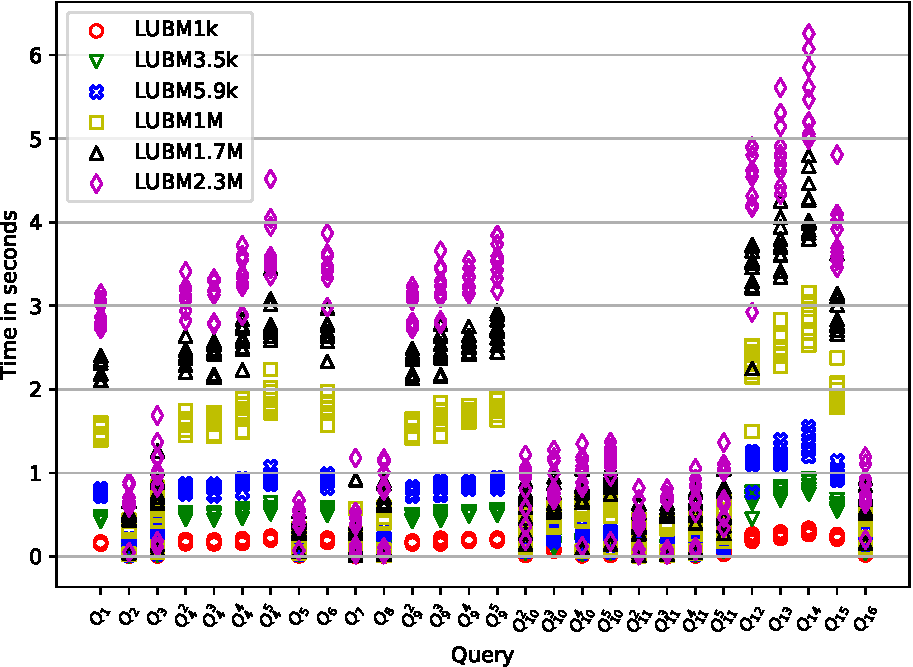
\includegraphics[width=0.6\textwidth]{data/LUBM_all.pdf}
   \caption{Index creation time for LUBM graphs}
   \label{fig:lubm_all_qs}
\end{figure}

Index creation time for each query on the real-world graphs is presented in Figure~\ref{fig:other_all_qs}.
We can see that querying small graphs requires more time than querying bigger graphs in some cases.
For example, conseder $Q_{10}^4$: querying the \textit{geospecies} graph (450k vertices) in some cases requires more time than querying of \textit{mappingbased\_properties} (8.3M vertices) and \textit{taxonomy} (5.7M vertices).
We conclude that the evaluation time depends on the inner structure of a graph.
On the other hand, \textit{taxonomy} querying in many cases requires significantly more time than for other graphs, while \textit{taxonomy} is not the biggest graph.
Finally, in most cases query execution lasts less than 10 seconds, even for bigger graphs, and no query requires more than 52.17 seconds.

\begin{figure}
    \centering
   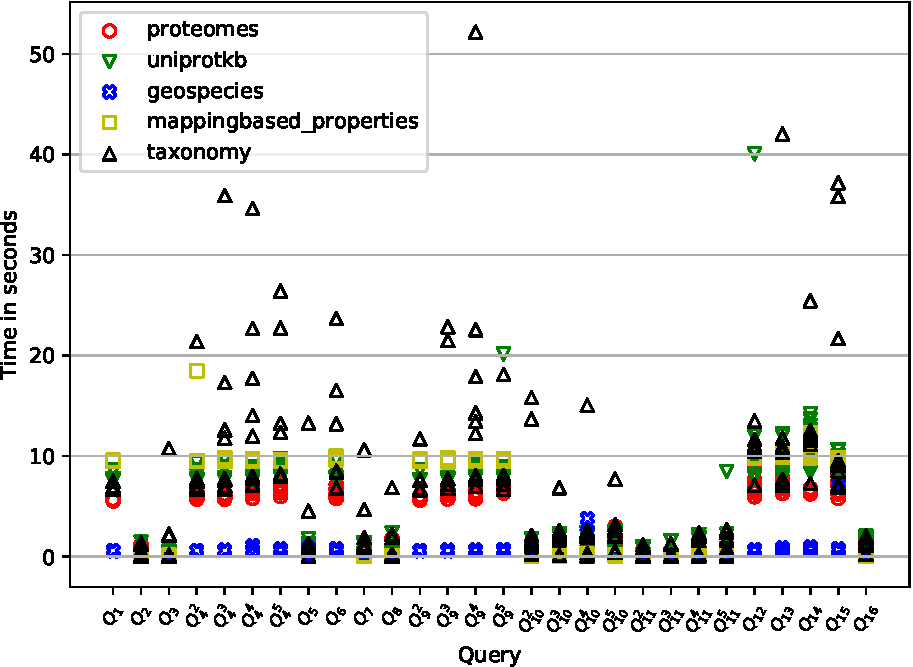
\includegraphics[width=0.6\textwidth]{data/other_all.pdf}
   \caption{Index creation time for real-world RDFs}
   \label{fig:other_all_qs}
\end{figure}

%We evaluate path extraction for queries which result in possibly long paths.
%Long paths usually require many iterations of transitive closure evaluation, thus we used the number of the iterations as a criterion to select the inputs for the evaluation.
%For each selected graph and query we measure paths extraction time for each reachable pair.
%Since the index can be reused from the previous step, we omit the time necessary to create the index.
%We limit by 10 the number of paths to extract.

%In Figures~\ref{fig:geo_tensors_rpq} and~\ref{fig:dbpedia_tensors_rpq} we show the time needed to extract a path of a specific length when only one path was extracted.
%The main observation is that time is linear on the path length, even if a generic path extraction procedure is used.

%\begin{figure}
%     \begin{subfigure}[b]{0.45\textwidth}
%         \centering
%         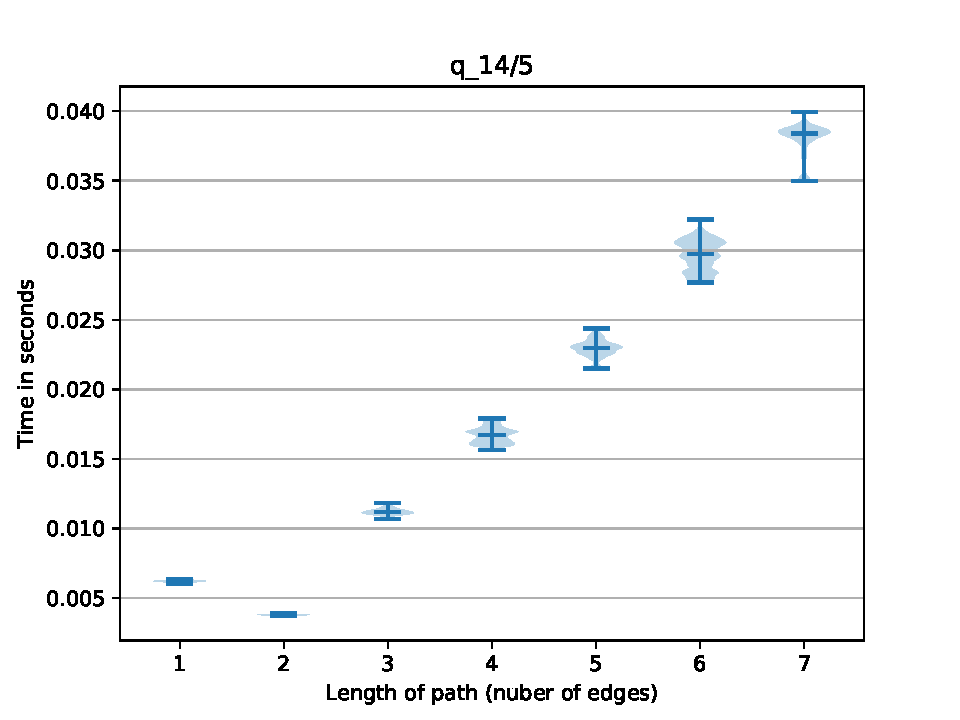
\includegraphics[width=\textwidth]{../paper/data/geo_rpq_single_path/q_14_5.pdf}
%         \caption{\footnotesize \textit{geospecies}, $Q_{14}$}
%         \label{fig:geo_tensors_rpq}
%     \end{subfigure}
%     ~\begin{subfigure}[b]{0.45\textwidth}
%         \centering
%         \includegraphics[width=\textwidth]{../paper/data/CF/Tensor_path/dbpedia_path_tensor.pdf}
%         \caption{\footnotesize \textit{mappingbased\_properties}, $Q_{4}^5$}
%         \label{fig:dbpedia_tensors_rpq}
%     \end{subfigure}\\
%     \begin{subfigure}[b]{0.45\textwidth}
%         \centering
%         \includegraphics[width=\textwidth]{../paper/data/CF/Matrix_CF/geo_path_matrix.pdf}
%         \caption{\footnotesize \textit{geospecies}, \textit{Geo}}
%         \label{fig:geo_matrix_cfpq}
%     \end{subfigure}
%     ~\begin{subfigure}[b]{0.45\textwidth}
%         \centering
%         \includegraphics[width=\textwidth]{../paper/data/CF/Tensor_path/geo_path_tensor.pdf}
%         \caption{\footnotesize \textit{geospecies}, \textit{Geo}}
%         \label{fig:geo_tensors_cfpq}
%     \end{subfigure}\\
%   \caption{Single path extraction for specific graph and query for our solution (\subref{fig:geo_tensors_rpq}, \%subref{fig:dbpedia_tensors_rpq}, \subref{fig:geo_tensors_cfpq}), and Azimov's (\subref{fig:geo_matrix_cfpq})}
%\end{figure}

\subsection{CFPQ Evaluation}

We evaluate the applicability of the proposed algorithm to CFPQ processing over real-world graphs on a number of classic cases and compare them with the Azimov's algorithm.
Currently only a single path version of Azimov's algorithm exists, and we use its implementation using PyGraphBLAS. Note that it is not trivial to compare our results with the state-of-the-art results provided by~\cite{10.1145/3398682.3399163} (Azimov's algorithm) because our algorithm computes significantly more information. While the state-of-the-art solution computes only reachability facts or a single-path semantics, our algorithm computes data necessary to restore all possible paths.

\subsubsection{Dataset}

We use CFPQ\_Data\footnote{CFPQ\_Data is a dataset for CFPQ evaluation which contains both synthetic and real-world data and queries \url{https://github.com/JetBrains-Research/CFPQ\_Data}. Access date: 07.07.2020.} dataset for evaluation.
Namely, we use relatively big RDF files and respective same-generation queries $G_1$~(Eq.~\ref{eqn:g_1}) and $G_2$~(Eq.~\ref{eqn:g_2}) which are used in other works for CFPQ evaluation.
We also use the $Geo$~(Eq.~\ref{eqn:geo}) query provided by~\cite{Kuijpers:2019:ESC:3335783.3335791} for \textit{geospecies} RDF.
Note that we use $\overline{x}$ notation in queries to denote the inverse of $x$ relation and the respective edge.
\begin{align}
\begin{split}
\label{eqn:g_1}
S \to & \overline{\textit{subClassOf}} \ \ S \ \textit{subClasOf} \mid \overline{\textit{type}} \ \ S \ \textit{type}\\   & \mid \overline{\textit{subClassOf}} \ \ \textit{subClasOf} \mid \overline{\textit{type}} \ \textit{type}
\end{split}
\end{align}
\begin{align}
\begin{split}
\label{eqn:g_2}
S \to \overline{\textit{subClassOf}} \ \ S \ \textit{subClasOf} \mid \textit{subClassOf}
\end{split}
\end{align}
\begin{align}
\begin{split}
\label{eqn:geo}
S \to & \textit{broaderTransitive} \ \  S \ \overline{\textit{broaderTransitive}} \\
      & \mid \textit{broaderTransitive} \ \  \overline{\textit{broaderTransitive}}
\end{split}
\end{align}
\begin{align}
\begin{split}
\label{eqn:ma}
S & \to \overline{d} \ V \ d \\
V & \to ((S?) \overline{a})^* (S?) (a (S?))^*
\end{split}
\end{align}

Additionally we evaluate our algorithm on memory aliases analysis problem: a well-known problem which can be reduced to CFPQ~\citep{Zheng:2008:DAA:1328897.1328464}.
To do it, we use some graphs built for different parts of Linux OS kernel (\textit{arch}, \textit{crypto}, \textit{drivers}, \textit{fs}) and the query $MA$~(Eq.~\ref{eqn:ma})~\citep{10.1145/3093336.3037744}.
The detailed data about all the graphs used is presented in Table~\ref{tbl:graphs_for_cfpq}.

{\setlength{\tabcolsep}{0.3em}
\begin{table}
    \centering
{
\caption{Graphs for CFPQ evaluation: \textit{bt} is broaderTransitive, \textit{sco} is subCalssOf}
\label{tbl:graphs_for_cfpq}
\scriptsize
\rowcolors{2}{black!2}{black!10}
\begin{tabular}{|l|c|c|c|c|c|c|c|}
\hline
Graph          & \#V       & \#E        & \#sco & \#type &\#bt & \#a  & \#d \\
\hline
\hline
eclass\_514en  & 239 111    & 523 727    & 90 512    & 72 517    &        ---        & ---  & --- \\
enzyme         & 48 815     & 109 695    & 8 163     & 14 989    &        ---        & ---  & --- \\
geospecies     & 450 609    & 2 201 532  & 0         & 89 062    &        20 867     & ---  & --- \\
go             & 272 770    & 534 311    & 90 512    & 58 483    &        ---        & ---  & --- \\
go-hierarchy   & 45 007     & 980 218    & 490 109   & 0         &        ---        & ---  & --- \\
taxonomy       & 5 728 398  & 14 922 125 & 2 112 637 & 2 508 635 &        ---        & ---  & --- \\
\hline
arch           & 3 448 422  & 5 940 484  &      ---     &  ---   &        ---        & 671 295 & 2 298 947 \\
crypto         & 3 464 970  & 5 976 774  &      ---     &  ---   &        ---        & 678 408 & 2 309 979 \\
drivers        & 4 273 803  & 7 415 538  &      ---     &  ---   &        ---        & 858 568 & 2 849 201 \\
fs             & 4 177 416  & 7 218 746  &      ---     &  ---   &        ---        & 824 430 & 2 784 943 \\
\hline
\end{tabular}
}
\end{table}
}
\subsubsection{Results}

We averaged the index creation time over 5 runs for both single-path Azimov's algorithm (\textbf{Mtx}) and the proposed algorithm (\textbf{Tns}) (see Table~\ref{tbl:CFPQ_index}).

{\setlength{\tabcolsep}{0.2em}
  \begin{table}
    \centering
    \caption{CFPQ evaluation results, time is measured in seconds}
    \label{tbl:CFPQ_index}
    \rowcolors{4}{black!2}{black!10}
    \small
    \begin{tabular}{| l | c | c | c | c | c | c | c | c |}
      \hline

      \multirow{2}{*}{Name}  & \multicolumn{2}{c|}{$G_1$} & \multicolumn{2}{c|}{$G_2$} & \multicolumn{2}{c|}{\textit{Geo}} & \multicolumn{2}{c|}{\textit{MA}}\\
      \cline{2-9}
                      & Tns    & Mtx    & Tns  & Mtx  & Tns   & Mtx   & Tns     & Mtx \\
      \hline
      \hline
      eclass\_514en   & 0.24   & 0.27   & 0.25 & 0.26 & ---   & ---   & ---     & ---\\
      enzyme          & 0.03   & 0.04   & 0.02 & 0.01 & ---   & ---   & ---     & ---\\
      geospecies      & 0.08   & 0.06   & $0^{*}$ & 0.01 & 26.12 & 16.58 & ---     & ---\\
      go-hierarchy    & 0.16   & 1.43   & 0.23 & 0.86 & ---   & ---   & ---     & ---\\
      go              & 1.56   & 1.74   & 1.21 & 1.14 & ---   & ---   & ---     & ---\\
      pathways        & 0.01   & 0.01   & 0.01 & 0.01 & ---   & ---   & ---     & ---\\
      taxonomy        & 4.81   & 2.71   & 3.75 & 1.56 & ---   & ---   & ---     & ---\\
      \hline
      arch            & ---    & ---    & ---  & ---  & ---   & ---   & 262.45  & 195.51  \\
      crypto          & ---    & ---    & ---  & ---  & ---   & ---   & 267.52  & 195.54  \\
      drivers         & ---    & ---    & ---  & ---  & ---   & ---   & 1309.57 & 1050.78 \\
      fs              & ---    & ---    & ---  & ---  & ---   & ---   & 470.49  & 370.73  \\
      \hline
    \end{tabular}
  \end{table}
}

Best to our knowledge, the proposed algorithm is the first algorithm that provides information about all paths of interest (Azimov's algorithm computes information about only one path).
The direct comparison with other solutions is impossible, and we just estimate the running time of our algorithm for a small number of cases.
Namely, we extract all paths with length not greater than 20 edges between all pairs of vertices from indeces created for graphs \textit{go} and \textit{eclass\_514en} and query $G_1$.
Paths extraction for one pair of vertices requires 2.64 seconds averaged over all pairs for \textit{go} graph. The~maximal time is 4699 seconds and 217737 paths were extracted during this time. The average number of paths between two vertices is 184.
For \textit{eclass\_514en} paths extraction for one pair of vertices requires 1.27 seconds averaged over all pairs. The~maximal time is 8.04 seconds and only one path is extracted during this time. The average number of paths between two vertices is 3.
We can see that paths can be extracted in a reasonable time, but a detailed analysis of paths extraction algorithm performance depends on graphs structure.

%Comparison of paths extraction is presented in Figures~\ref{fig:geo_matrix_cfpq} and~\ref{fig:geo_tensors_cfpq}.
%While both methods demonstrate linear time on the length of the extracted path, our generic solution is more than 1000 times slower than Azimov's single path extraction procedure.
%We conclude that current generic all-path extraction procedure is not optimal for single path extraction.

\subsection{Conclusion}

We conclude that the proposed algorithm is applicable to real-world data processing: the algorithm allows one to solve both the reachability problem and to extract paths of interest in a reasonable time even using naive implementation.
While index creation time (reachability query evaluation) is comparable with other existing solutions, paths extraction procedure should be improved in the future. However, the state-of-the-art solution computes only reachability facts or a single-path semantics, whereas our algorithm computes data necessary to restore all possible paths (all-paths semantics).
Finally, a detailed comparison of the proposed solution with other algorithms for CFPQ and RPQ is required.

To summarize the overall evaluation, the proposed algorithm is applicable to both RPQ and CFPQ over real-world graphs.
Thus, the proposed solution is a promising unified algorithm for both RPQ and CFPQ evaluation.

\section{Conclusion}

Conclusion, current state, results.

Future work. Library extension up to full GraphBLAS API implementation.

LaGraph on F\# .NET.

Evaluation. Comparison with other implementations on different devices.
Manual implementation versus translation.  

Another direction of future work is Brahma.FSharp improvements. 
First of all, it is necessary to support discriminated unions to make it possible to express custom semirings such as \texttt{Min-Plus}, as presented in listing~\ref{lst_example}. 

Also, it is necessary to add high-level abstractions for asynchronous programming, and for multi-GPU programming.
Such mechanisms can be naturally expressed in F\# with native primitives for asynchronous programming.

fusion and other optimizations.

\setmonofont[Mapping=tex-text]{CMU Typewriter Text}
\bibliographystyle{ugost2008ls}
\bibliography{diploma.bib}
\end{document}
